\documentclass[notes,blackandwhite,mathsans,usenames,dvipsnames]{beamer}

\usepackage{amsmath}
\usepackage{amssymb}
\usepackage{graphicx}
\usepackage{fancybox}
\usepackage{booktabs}
\usepackage{multirow,multicol,pxfonts}
\usepackage{cmbright}
\usepackage{xcolor}
\usepackage{color}
\usepackage{enumitem}
\usepackage{animate}
\usepackage{changepage}
\usepackage{cmbright}

\usepackage[T1]{fontenc}
\fontencoding{T1}  
\usepackage[utf8]{inputenc}


\usefonttheme{default}
\setbeamercovered{invisible}
\beamertemplatenavigationsymbolsempty

\makeatletter
\setbeamertemplate{footline}
{
  \leavevmode
  \hbox{
  \begin{beamercolorbox}[wd=0.97\paperwidth,ht=2.25ex,dp=2ex,right]{}
{\color{gre} \insertframenumber{} / \inserttotalframenumber}
  \end{beamercolorbox}}%
}


\definecolor{yel}{HTML}{FED500}
\definecolor{gre}{HTML}{4EB1AD}
\definecolor{blu}{HTML}{865BB8}

\setbeamercolor{frametitle}{fg=gre}
\AtBeginDocument{\color{blu}}
\setbeamertemplate{itemize item}[triangle]



\begin{document}
%\fontfamily{pag}\selectfont
%\setbeamerfont{title}{family=\fontfamily{pag}\selectfont}
%\setbeamerfont{frametitle}{family=\fontfamily{pag}\selectfont}
%\setbeamerfont{framesubtitle}{family=\fontfamily{pag}\selectfont}






{\setbeamercolor{background canvas}{bg=gre}
\begin{frame}

\vspace{1cm}
\begin{tabular}{rl}
&\textbf{\LARGE\color{yel} Macroeconometrics}\\[8ex]
\textbf{\large\color{yel} Lecture 23}&\textbf{\large\color{blu}Less than $\mathbf{2^{\circ}}$C warming by 2100 unlikely}\\
&\textbf{\large\color{blu}-- partial reproduction}\\[6ex]
&{\large\color{white} Topics in Climate Change}\\
&{\large\color{white} Forecasting CO$_2$ Emissions for the 21st Century}\\[7ex]
&\textbf{Tomasz Wo\'zniak}\\[2ex]
%&\colorbox{blu}{\textit{\small\color{white}\href{https://www.schoolstrike4climate.com/may21}{\#CLIMATESTRIKE MAY21}}}
%&{\small\color{white} Department of Economics}\\
%&{\small\color{white}University of Melbourne}
\end{tabular}

\end{frame}
}


{\setbeamercolor{background canvas}{bg=gre}
\begin{frame}

\vspace{1cm}\textbf{\color{yel}The data, the model, and prior assumptions}

\bigskip\textbf{\color{blu}Matrix notation and MCMC sampler}

\bigskip\textbf{\color{blu}Estimation results}

\bigskip\textbf{\color{yel}Probabilistic predictions}



\vspace{2cm} Lecture is based on: \footnotesize

\smallskip{\color{yel} 
Raftery, Zimmer, Frierson, Startz, Liu (2017), Less than $2^{\circ}$C warming by 2100 unlikely, Nature Climate Change, Vol.~7.
}

\normalsize\bigskip
Materials: \footnotesize

\smallskip{\color{yel}A zip file} \texttt{L23mcxs-all.zip} {\color{yel}for the reproduction of the results}

\end{frame}
}




{\setbeamercolor{background canvas}{bg=yel}
\begin{frame}

\begin{adjustwidth}{-0.5cm}{0cm}
\vspace{8.3cm}\Large
\textbf{{\color{blu}The data,} {\color{gre}the model, and prior assumptions}}
\end{adjustwidth}

\end{frame}
}





\begin{frame}{The data: GDP data}

\begin{center}
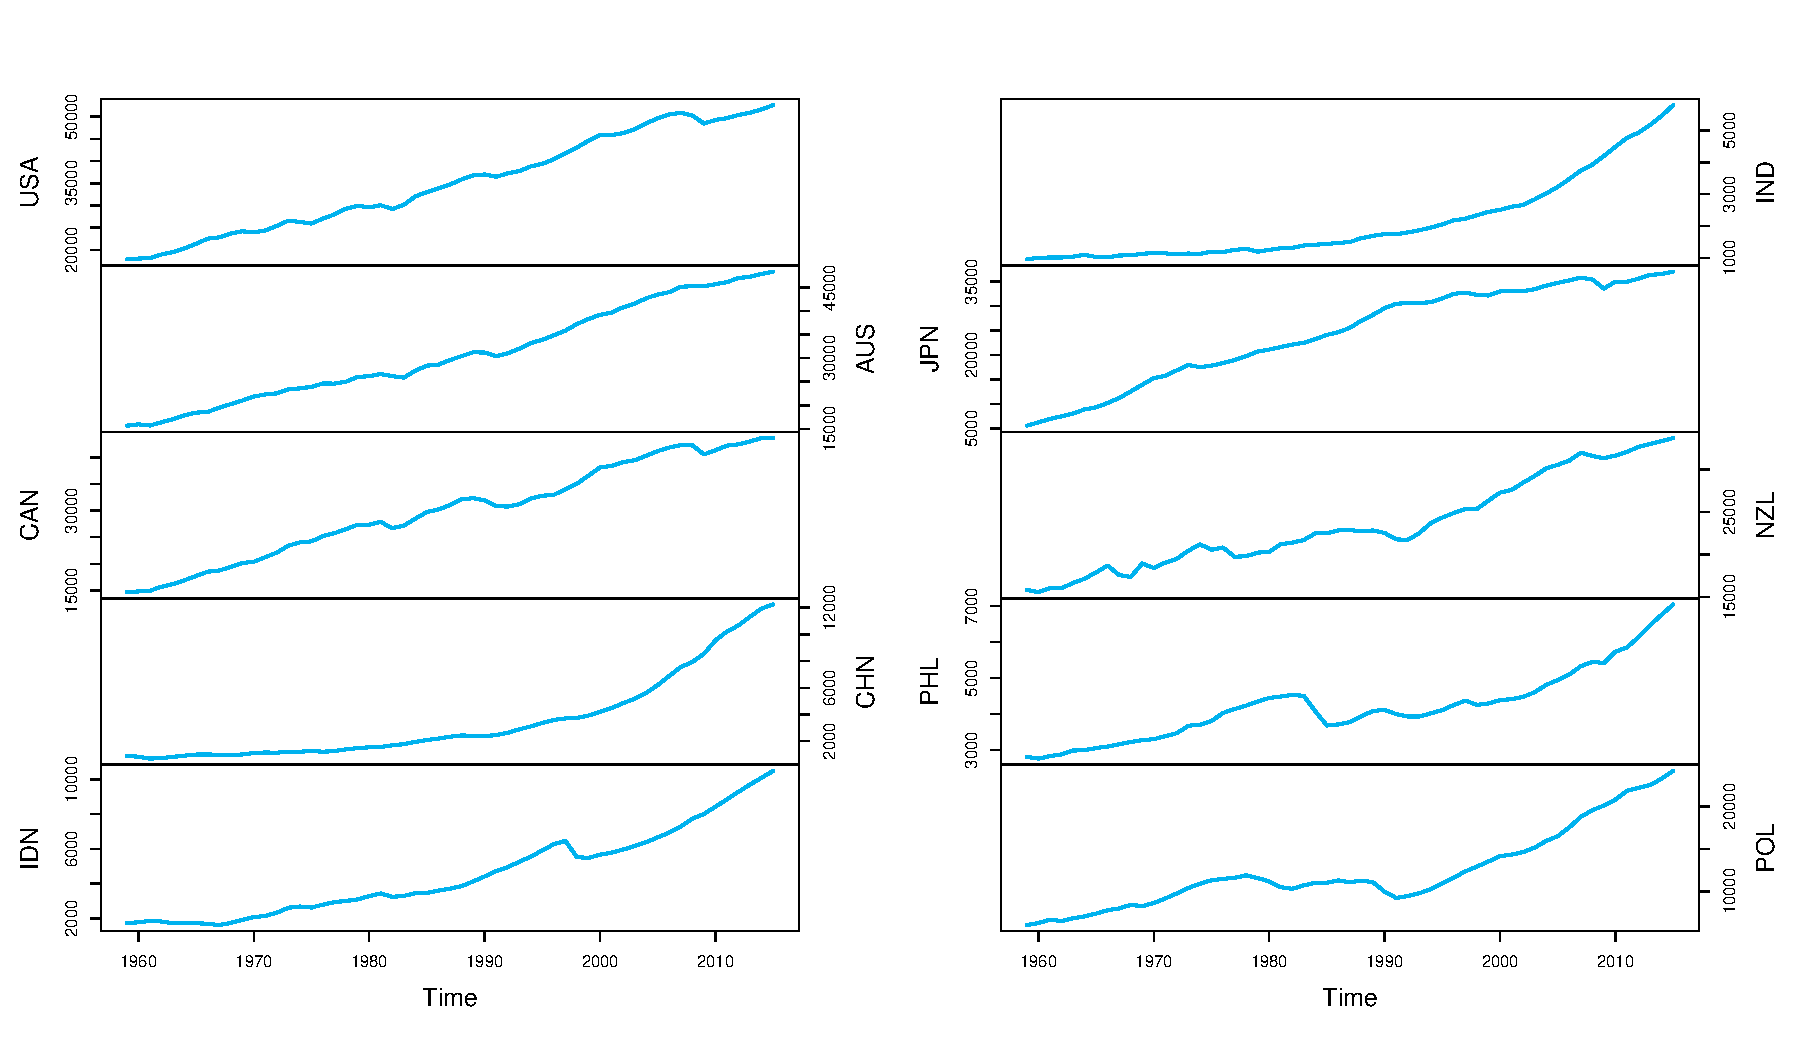
\includegraphics[scale=0.36]{./01empirical/grph-GDP.pdf}

\small
{\color{gre}Annual data from 1959--2015 ($T=56$ of differentiated series, $N=10$)\\
Model applied to logarithms of the original data\\
Source: data files of Raftery et al. (2017)}
\end{center}
\end{frame}



\begin{frame}{The data: carbon intensity}

\begin{center}
\begin{multicols}{2}
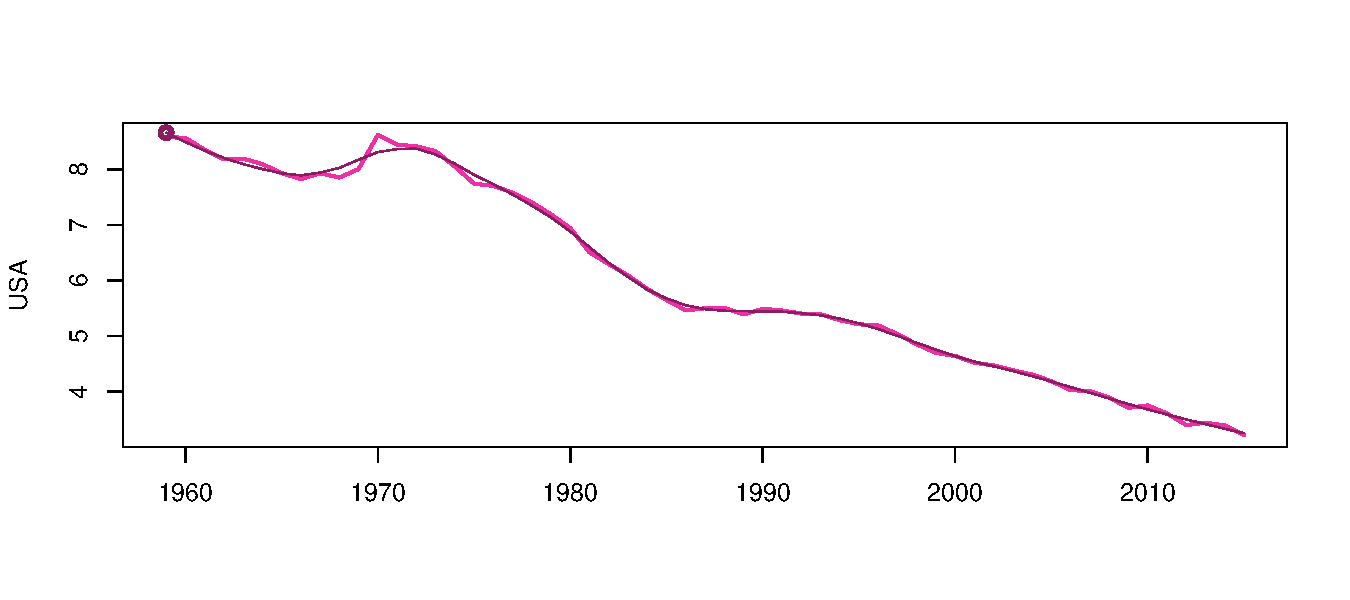
\includegraphics[trim=0cm 2.55cm 1cm 2.05cm, clip=true, scale=0.22]{./01empirical/grph-Intensity-1.pdf}
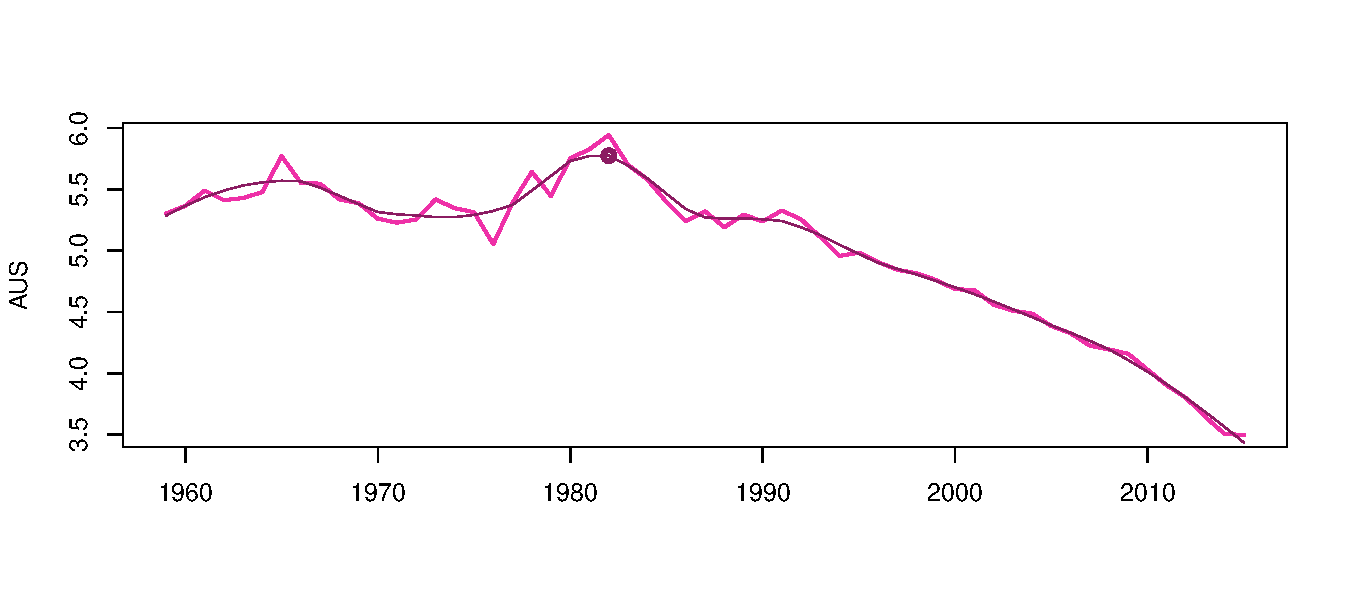
\includegraphics[trim=0cm 2.55cm 1cm 2.15cm, clip=true, scale=0.22]{./01empirical/grph-Intensity-2.pdf}
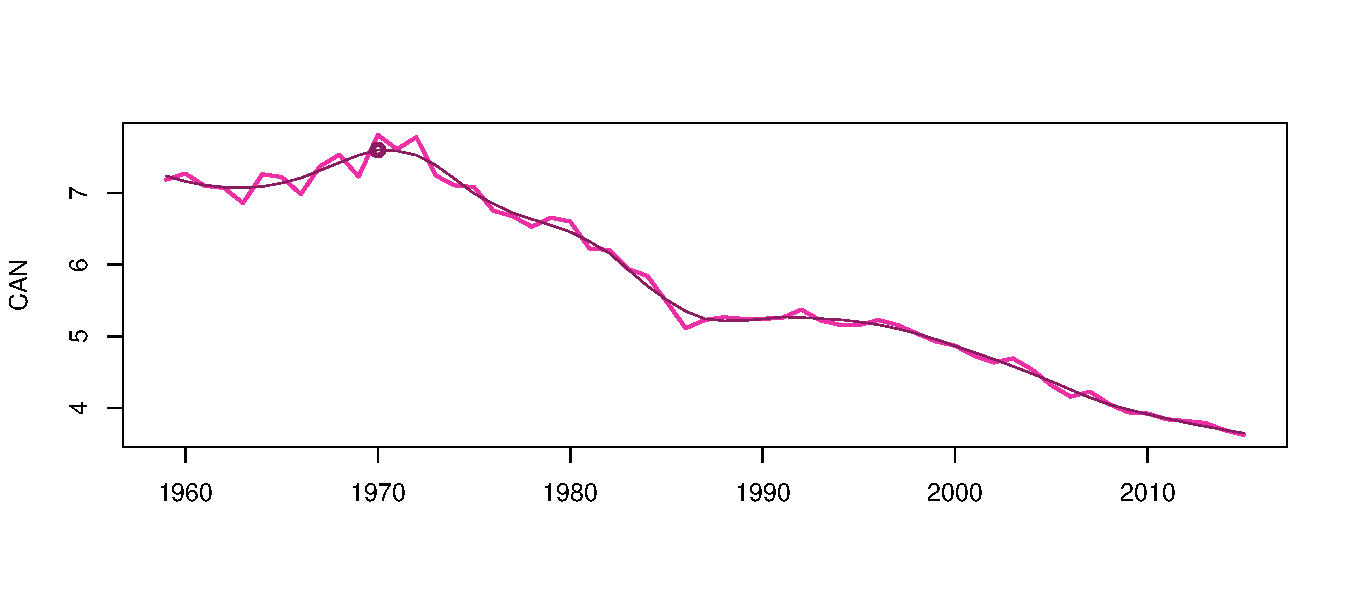
\includegraphics[trim=0cm 2.55cm 1cm 2.15cm, clip=true, scale=0.22]{./01empirical/grph-Intensity-3.pdf}
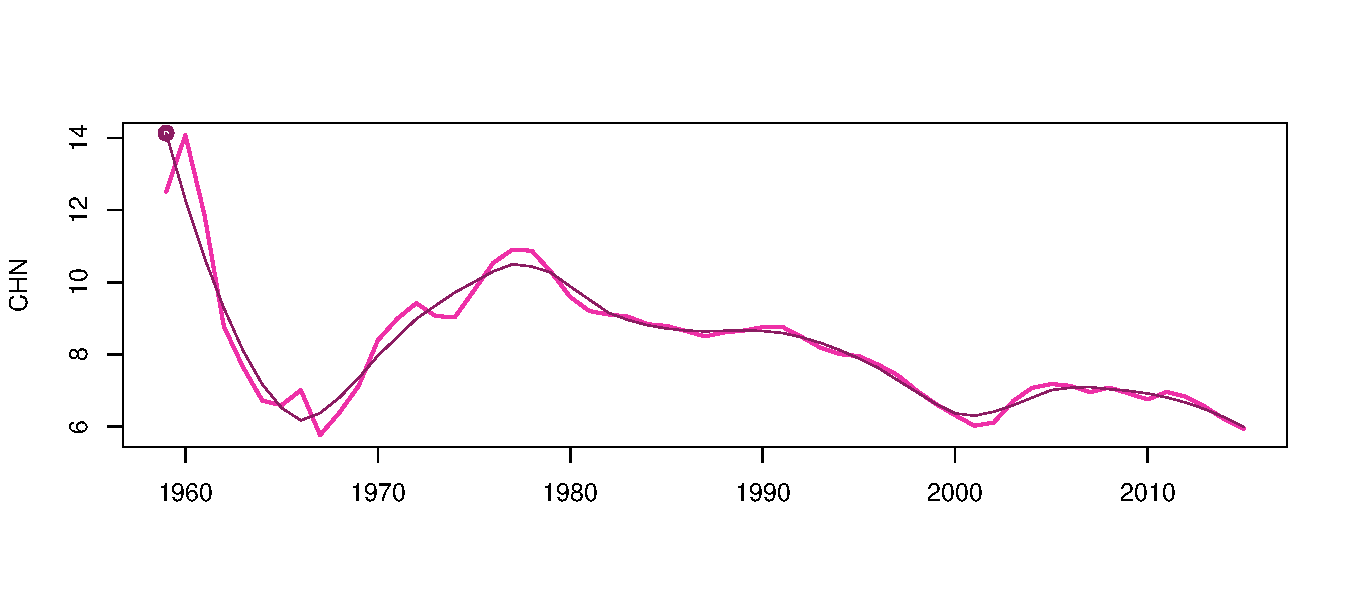
\includegraphics[trim=0cm 2.55cm 1cm 2.15cm, clip=true, scale=0.22]{./01empirical/grph-Intensity-4.pdf}
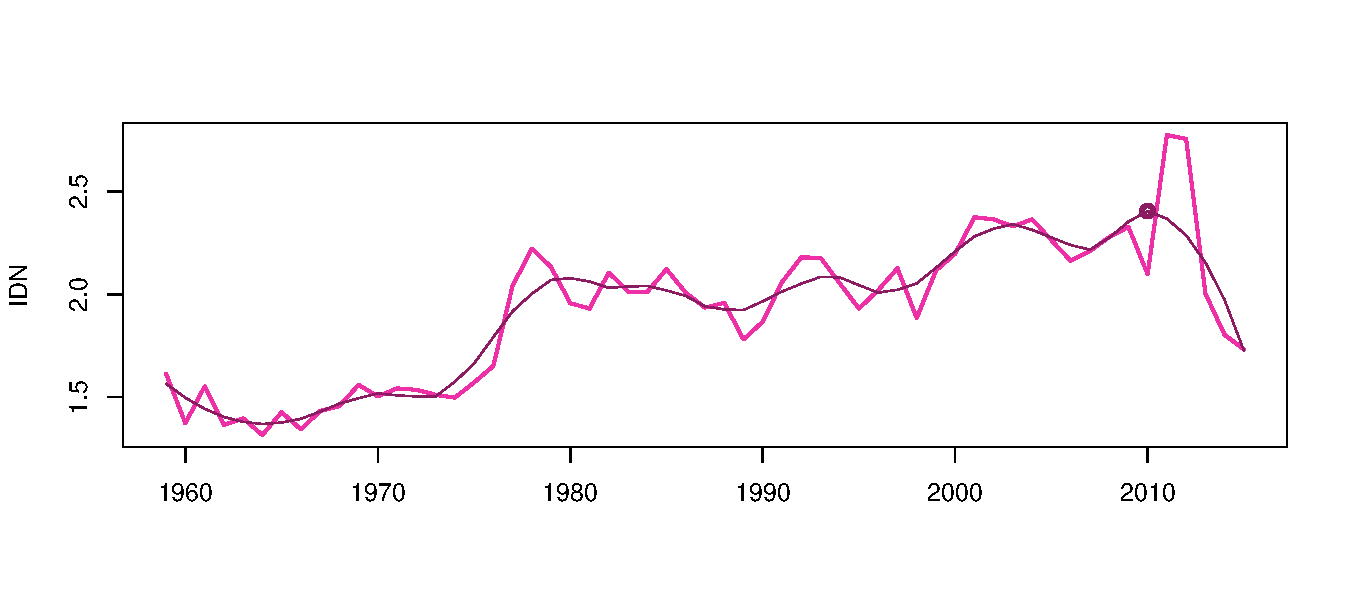
\includegraphics[trim=0cm 1.5cm 1cm 2.15cm, clip=true, scale=0.22]{./01empirical/grph-Intensity-5.pdf}


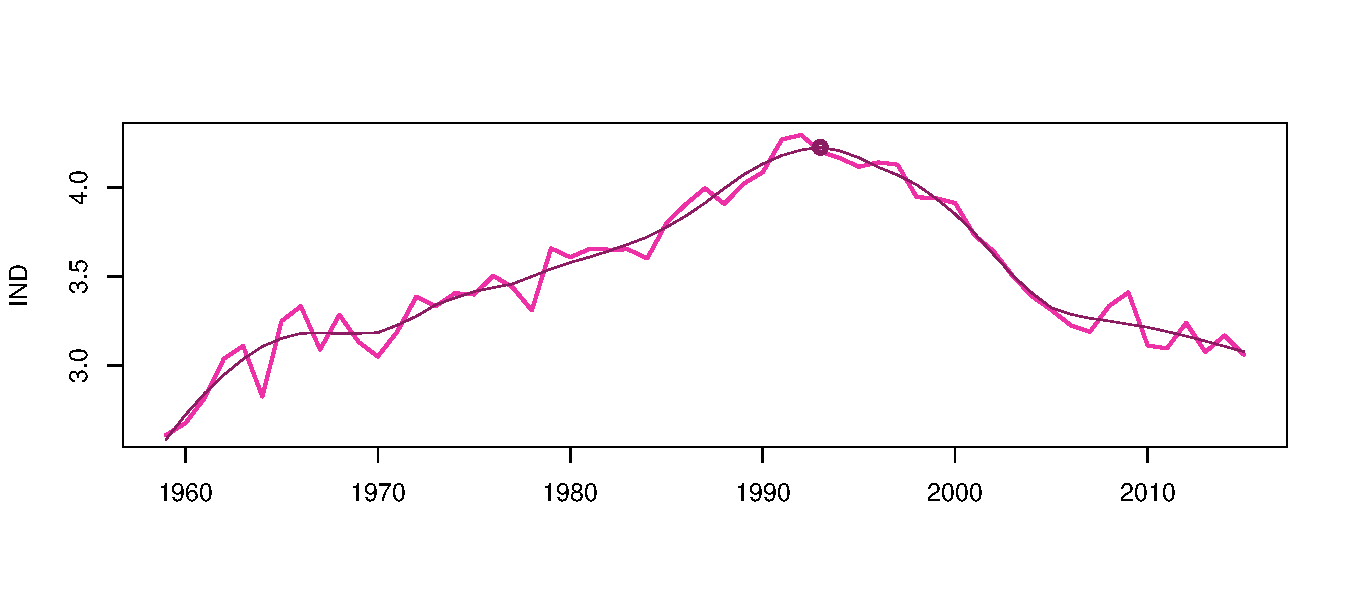
\includegraphics[trim=0cm 2.55cm 1cm 2.05cm, clip=true, scale=0.22]{./01empirical/grph-Intensity-6.pdf}
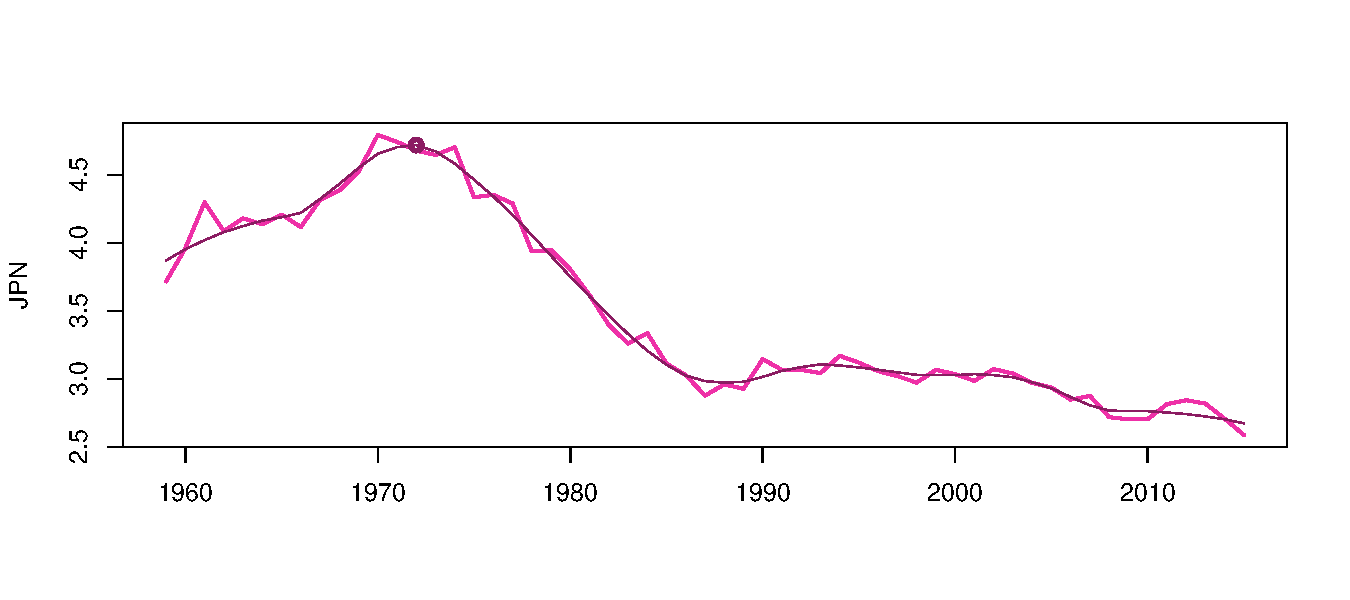
\includegraphics[trim=0cm 2.55cm 1cm 2.15cm, clip=true, scale=0.22]{./01empirical/grph-Intensity-7.pdf}
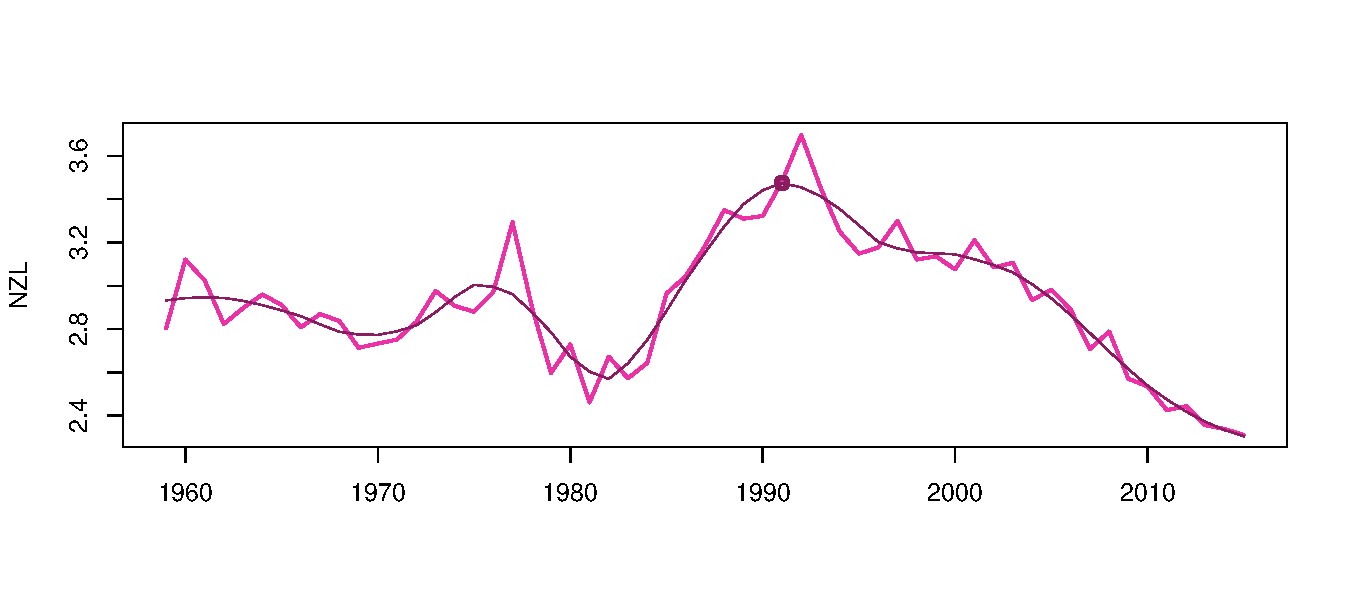
\includegraphics[trim=0cm 2.55cm 1cm 2.15cm, clip=true, scale=0.22]{./01empirical/grph-Intensity-8.pdf}
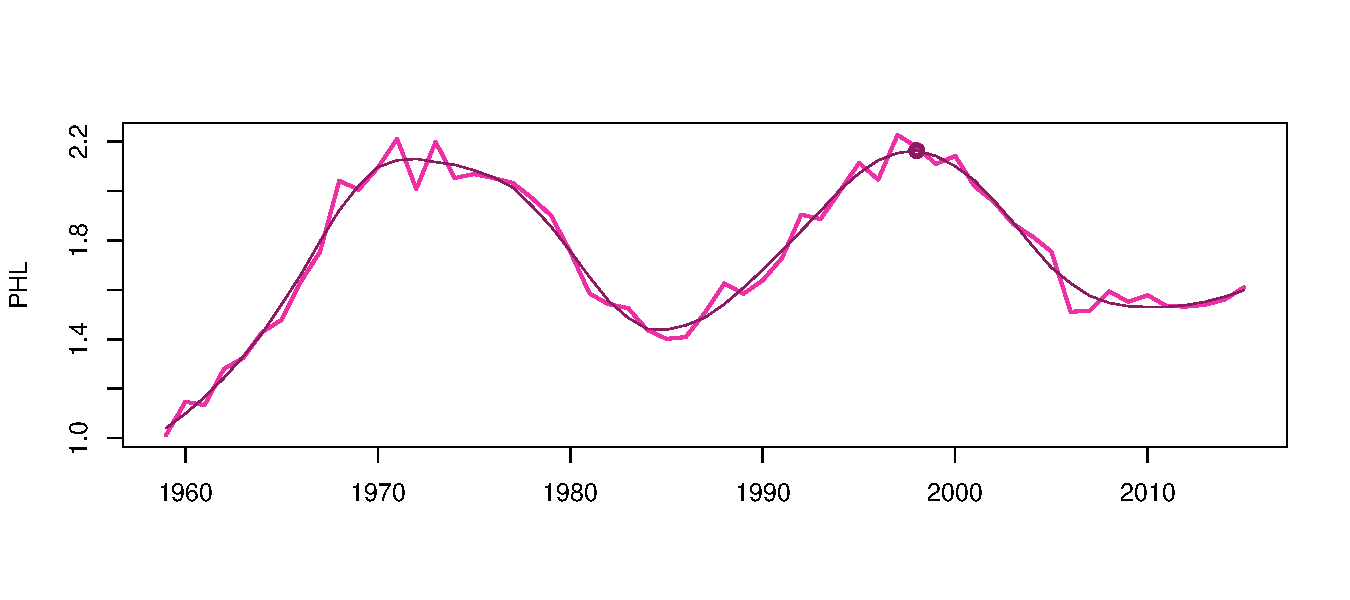
\includegraphics[trim=0cm 2.55cm 1cm 2.15cm, clip=true, scale=0.22]{./01empirical/grph-Intensity-9.pdf}
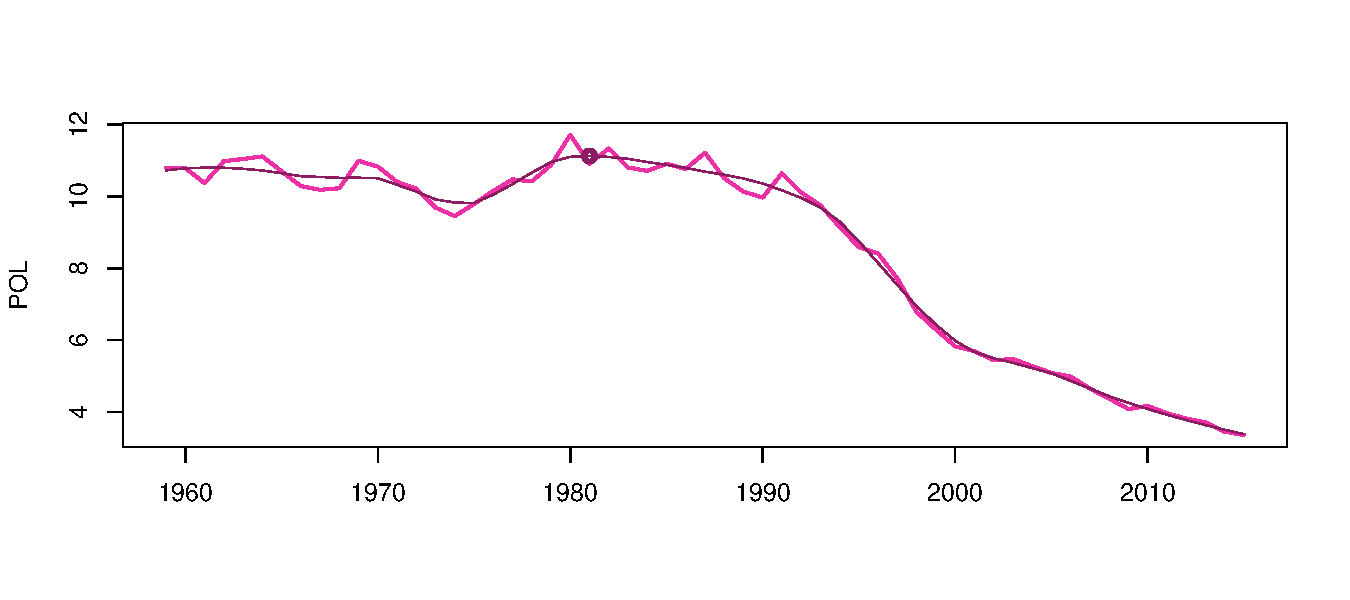
\includegraphics[trim=0cm 1.5cm 1cm 2.15cm, clip=true, scale=0.22]{./01empirical/grph-Intensity-10.pdf}

\end{multicols}
\small
{\color{gre}The data, loess smoothed values, and cut-off dates}
\end{center}
\end{frame}








\begin{frame}{Model and prior assumptions}

\textbf{Model for the frontier economy -- prior distributions.}
\begin{align*}
F_t &= F_{t-1} + \gamma +\gamma_{pre 1973}\mathcal{I}(t\leq 1973) + \epsilon_t^{(f)}\\
\epsilon_t^{(f)} &\sim\mathcal{N}\left( 0,\sigma_f^2 \right)\\[2ex]
\gamma &\sim\mathcal{U}[0,1]\\
\gamma_{pre 1973} &\sim\mathcal{U}[-0.1,0.1]\\
\sigma_f^2 &\sim\mathcal{IG}2(\hat{s}^2,3)
\end{align*}

\end{frame}



\begin{frame}{Model and prior assumptions}

\textbf{Model for other economies -- prior distributions.}
\begin{align*}
(F_t - G_{c.t}) &= \phi_c(F_{t-1}- G_{c.t-1}) + \epsilon_{c.t}^{(g)}\\
\epsilon_{c.t}^{(g)} &\sim\mathcal{N}\left( 0,\sigma_{g.c}^2 \right)\\[2ex]
\phi_c|\mu_\phi, \sigma_\phi^2 &\sim\mathcal{TN}_{[0,1]}\left(\mu_\phi, \sigma_\phi^2\right)\\
\mu_\phi &\sim\mathcal{U}[0,1] \\
\sigma_\phi^2 &\sim \mathcal{U}[0,1]\\[2ex]
\sigma_{g.c}^2|\underline{s} &\sim\mathcal{IG}2\left(\underline{s},3\right)\\
\underline{s} &\sim\mathcal{G}\left( 1,1 \right)
\end{align*}

\end{frame}




\begin{frame}{Model and prior assumptions}

\textbf{Model for carbon intensity.}\small
\begin{align*}
\tau_{c.t} &= \eta (t-\bar{t}) + \beta \tau_{c.t-1} - \delta_{c} + \rho\frac{\sigma_c}{\sigma_{g.c}}\epsilon_{c.t}^{(g)}   + \epsilon_{c.t}\\
\epsilon_{c.t} &\sim\mathcal{N}\left( 0,\sigma_{c}^2 \right)\\[2ex]
\eta&\sim \mathcal{N}\left( 0.1,0.01 \right)\\
\beta&\sim \mathcal{U}[0,1]\\
\rho&\sim\mathcal{U}[-1,1]\\[1ex]
\delta_c|\mu_\delta,\sigma_\delta^2&\sim\mathcal{N}\left(\mu_\delta,\sigma_\delta^2\right) \\
\mu_\delta&\sim\mathcal{N}(0,1) \\
\sigma_\delta^2 &\sim\mathcal{IG}2(1,1) \\[1ex]
\sigma_{c}^2|\underline{s}_\sigma &\sim\mathcal{IG}2\left(\underline{s}_\sigma,3\right)\\
\underline{s}_\sigma &\sim\mathcal{G}(1,1)
\end{align*}

\end{frame}








{\setbeamercolor{background canvas}{bg=blu}
\begin{frame}

\begin{adjustwidth}{-0.5cm}{0cm}
\vspace{8.3cm}\Large
\textbf{{\color{gre}Matrix notation} {\color{yel}and Gibbs sampler}}
\end{adjustwidth}

\end{frame}
}



\begin{frame}{Metropolis-Hastings sampler}

\begin{description}
\item[an MCMC] method for sampling from the posterior distribution of parameters $\theta$
\item[requires] only an ordinate of the kernel of the posterior density
$$ k(\theta) = L(\theta,\mathbf{y})p(\theta) $$
\item[relies on] the specification of a candidate drawing density
$$ \theta^*\sim q(\theta) $$
\item[accept] the candidate draw $\theta^*$ with probability
$$ \min\left\{1, \frac{k(\theta^*)q(\theta^*)}{k(\theta^{(s-1)})q(\theta^{(s-1)})}\right\} $$
\item[Gibbs sampler] is its special case with acceptance probability 1
\end{description}

\end{frame}



\begin{frame}{Metropolis-Hastings sampler}

\begin{description}
\item[Due to a non-standard] form of dependence in equation
$$ \tau_{c.t} = \eta (t-\bar{t}) + \beta \tau_{c.t-1} - \delta_{c} + \rho\frac{\sigma_c}{\sigma_{g.c}}\epsilon_{c.t}^{(g)}   + \epsilon_{c.t} $$
the full conditional posterior distributions are non-standard 

\smallskip\item[Estimation strategy:] derive the full conditional posterior densities for all of the parameters as if $\frac{\sigma_c}{\sigma_{g.c}}\epsilon_{c.t}^{(g)}$ was a fixed regressor and use these densities as candidate drawing densities. Accept or reject the candidate draws with appropriate probabilities.

\end{description}

\end{frame}




\begin{frame}{Uniform prior distribution}

\begin{description}
\item[Uniform prior] distributions help to impose restrictions
\item[Density function] of a uniform distribution $\mathcal{U}(a,b)$ does not depend o the random variable and is equal to $(b-a)^{-1}$
\item[Full conditional posterior] distribution for a parameter $\theta\sim\mathcal{U}(a,b)$ is a truncated density, for instance:
\begin{align*}
L(\theta|\mathbf{y}) &= \mathcal{N}(\tilde{\theta},\tilde{V}_\theta)\\
\theta &= \mathcal{U}(a,b)\\
\downarrow&\\
p(\theta|\mathbf{y},\dots) &= \mathcal{N}(\tilde{\theta},\tilde{V}_\theta)\mathcal{I}(\theta\in[a,b])
\end{align*}
\end{description}

\end{frame}





\begin{frame}{Hierarchical prior distributions: normal}

\begin{align*}
\theta|\mu_\theta,\sigma^2_\theta &\sim\mathcal{N}(\mu_\theta,\sigma^2_\theta)\\[1ex]
\mu_\theta &\sim\mathcal{N}(\mu_\mu,\sigma^2_\mu)\\
\sigma^2_\theta&\sim\mathcal{IG}2(s_\theta,\nu_\theta)\\[1ex]
\downarrow&\\[1ex]
\mu_\theta|\theta,\sigma^2_\theta,\mu_\mu,\sigma^2_\mu &\sim\mathcal{N}\left((\sigma_\theta^{-2} + \sigma_\mu^{-2})^{-1}(\sigma_\theta^{-2}\theta + \sigma_\mu^{-2}\mu_\mu)
,(\sigma_\theta^{-2} + \sigma_\mu^{-2})^{-1}\right)\\[1ex]
\sigma^2_\theta|\theta,\mu_\theta,s_\theta,\nu_\theta &\sim\mathcal{IG}2\left( s_\theta + (\theta-\mu_\theta)^2, \nu_\theta+1\right)
\end{align*}

\end{frame}


\begin{frame}{Hierarchical prior distributions: inverse gamma 2}

\begin{align*}
\sigma^2|\underline{s} &\sim\mathcal{IG}2(\underline{s},\nu)
\propto \underline{s}^{\frac{\nu}{2}}\left(\sigma^2\right)^{-\frac{\nu+2}{2}}\exp\left\{-\frac{1}{2}\frac{\underline{s}}{\sigma^2} \right\}
\\[1ex]
\underline{s}&\sim\mathcal{G}(s,a)
\propto \underline{s}^{a-1}\exp\left\{ -\frac{\underline{s}}{s}\right\}
\\[1ex]
\downarrow&\\[1ex]
\underline{s}|\sigma^2 &\sim\mathcal{G}\left( \left(s^{-1} + 0.5\sigma^{-2}\right)^{-1}, \frac{\nu}{2}+a	\right)
\end{align*}

\end{frame}








\begin{frame}{Model for the frontier economy: matrix notation.}

\begin{align*}
F &= X_F \gamma + \epsilon^{(f)}\\
\epsilon^{(f)} &\sim\mathcal{N}_T\left( \mathbf{0}_T,\sigma_f^2I_T \right)\\[2ex]
\gamma &\sim\mathcal{U}[0,1]\\
\gamma_{pre 1973} &\sim\mathcal{U}[-0.1,0.1]\\
\sigma_f^2 &\sim\mathcal{IG}2(\hat{s}^2,3)
\end{align*}

\footnotesize
$$
\underset{56\times1}{F}=\begin{bmatrix} F_2-F_1\\ \vdots \\ F_T-F_{T-1} \end{bmatrix},\quad
\underset{56\times2}{X_F}=\begin{bmatrix} \imath_{14} & \imath_{14}\\  \imath_{42} & \mathbf{0}_{42}  \end{bmatrix},\quad
\underset{56\times1}{\epsilon^{(f)}}=\begin{bmatrix} \epsilon^{(f)}_1\\ \vdots \\ \epsilon^{(f)}_T \end{bmatrix},\quad
\underset{2\times1}{\gamma}=\begin{bmatrix} \gamma  \\ \gamma_{pre1973} \end{bmatrix},\quad
$$

\end{frame}




\begin{frame}{Model for the frontier economy: MCMC sampler.}

\begin{align*}
\gamma|F, X_F,\sigma_f^2 &\sim\mathcal{N}_2\left( \bar{\gamma}, \bar{V}_{\gamma} \right)\mathcal{I}\left(\begin{array}{c}\gamma\in [0,1]\\ \gamma_{pre1973}\in[-.1,.1]\end{array}\right)\\[1ex]
\bar{V}_{\gamma} &= \left( \sigma_f^{-2}X_F'X_F \right)^{-1} \\
\bar{\gamma}&= \left( X_F'X_F \right)^{-1}X_F' F \\[2ex]
\sigma_f^2|F, X_F,\gamma &\sim\mathcal{IG}2\left( \bar{s}_f, \bar{\nu}_f \right)\\[1ex]
\bar{s}_f &= \hat{s}^2 + (F-X_F \gamma)'(F-X_F \gamma) \\
\bar{\nu}_f &= T+3
\end{align*}

\end{frame}




\begin{frame}{Model for other economies -- matrix notation.}

\begin{align*}
G &= X_G \phi + \epsilon^{(g)}\\
\epsilon^{(g)} &\sim\mathcal{N}_{(N-1)T}\left( \mathbf{0}_{(N-1)T}, \Sigma_G \right)\\
\Sigma_G &= \text{diag}\left(\sigma_{g.2}^2,\dots,\sigma_{g.N}^2\right)\otimes I_T\\[2ex]
\phi|\mu_\phi,\sigma_\phi^2 &\sim\mathcal{N}_{N-1}\left( \mu_\phi\imath_{N-1}, \sigma_\phi^2 I_{N-1} \right)\\
\mu_\phi &\sim\mathcal{U}[0,1]\\
\sigma_\phi^2 &\sim\mathcal{U}[0,1]\\
\sigma_{g.c}^2|\underline{s} &\sim\mathcal{IG}2(\underline{s},3)\\
\underline{s}&\sim\mathcal{G}(1,1)
\end{align*}

\end{frame}




\begin{frame}{Model for other economies -- matrix notation.}

\scriptsize
$$
\underset{(N-1)T\times1}{G}=\begin{bmatrix} F_2-G_{2.1}\\ \vdots \\ F_T-G_{2.T} \\ \vdots\\ F_2-G_{N.2}\\ \vdots \\ F_T-G_{N.T}  \end{bmatrix},\quad
\underset{(N-1)T\times1}{\epsilon^{(g)}}=\begin{bmatrix} \epsilon^{(g)}_{2.2}\\ \vdots \\ \epsilon^{(g)}_{2.T} \\ \vdots\\ \epsilon^{(g)}_{N.2}\\ \vdots \\ \epsilon^{(g)}_{N.T}  \end{bmatrix},\quad
\underset{N-1\times 1}{\phi} = \begin{bmatrix} \phi_2\\ \vdots \\ \phi_N \end{bmatrix}
$$
$$
\underset{(N-1)T\times (N-1)}{X_G}=\begin{bmatrix} F_1-G_{2.1}&...&0 \\ \vdots&&\vdots \\ F_{T-1}-G_{2.T-1}&...&0 \\ \vdots&&\vdots \\ 0&...& F_1-G_{N.1}\\ \vdots&&\vdots \\ 0&...&F_{T-1}-G_{N.T-1}  \end{bmatrix}\quad
$$
\end{frame}



\begin{frame}{Model for other economies -- MCMC sampler.}

\footnotesize
\begin{align*}
\phi|G,X_G,\sigma_g^2,\mu_\phi,\sigma_\phi^2 &\sim\mathcal{N}_{N-1}\left(\bar{\phi},\bar{V}_\phi\right)\mathcal{I}\left(\phi_c\in[0,1]\right)\\
\bar{V}_\phi &= \left(X_G'\Sigma_G^{-1}X_G + \sigma_\phi^{-2}I_{N-1}\right)^{-1}\\
\bar{\phi}&= \bar{V}_\phi\left( X_G'\Sigma_G^{-1}G + \sigma_\phi^{-2}\mu_\phi \imath_{N-1} \right)\\[2ex]
\sigma_{g.c}^2|G,X_G,\underline{s} &\sim\mathcal{IG}2(\bar{s}_{g.c},\bar{\nu}_{g.c})\\
\bar{s}_{g.c} &=\underline{s} + (G-X_G \phi)'(G-X_G \phi) \\
\bar{\nu}_{g.c} &=T+3 \\[2ex]
\mu_\phi|\phi,\sigma_\phi^2&\sim\mathcal{N}_{N-1}\left(\bar{\mu}_\phi,\bar{V}_{\mu_\phi}\right)\mathcal{I}\left(\mu_\phi\in[0,1]\right)\\
\bar{V}_{\mu_\phi}&=\sigma_\phi^2/(N-1)\\
\bar{\mu}_\phi&=\bar{V}_{\mu_\phi}\sigma_\phi^{-2}\imath_{N-1}'\phi\\[2ex]
\sigma_\phi^2|\phi,\mu_\phi&\sim\mathcal{IG}2\left(\bar{s}_\phi, N-3\right)\mathcal{I}\left(\sigma_\phi^2\in[0,1]\right)\\
\bar{s}_\phi&= (\phi-\mu_\phi\imath_{N-1})'(\phi-\mu_\phi\imath_{N-1})\\
\underline{s}|\sigma_g^2&\sim\mathcal{G}\left(\left( 1 + .5\sum_c\sigma_{g.c}^{-2} \right)^{-1} , 1.5(N-1)+1 \right)
\end{align*}

\end{frame}



\begin{frame}{Model for carbon intensity -- matrix notation.}

\small
\begin{align*}
\tau &= X_\tau \beta_\tau + \epsilon\\
\epsilon &\sim\mathcal{N}_{(\sum_{c=1}^NT_c)}\left(\mathbf{0},\Sigma  \right)\\[2ex]
\beta_\tau|\mu_\delta,\sigma_\delta^2 &\sim\mathcal{N}_{N+3}\left(\underline{\mu}_\beta, \underline{V}_\beta\right)\mathcal{I}\left(\begin{array}{c} \beta\in[0,1]\\ \rho\in[-1,1] \end{array}\right)\\
\mu_\delta&\sim\mathcal{N}(0,1)\\
\sigma_\delta^2&\sim\mathcal{IG}2(1,1)\\[1ex]
\sigma_c^2|\underline{s}_\sigma&\sim\mathcal{IG}2(\underline{s}_\sigma,3)\\
\underline{s}_\sigma&\sim\mathcal{G}(1,1)\\[2ex]
\underline{\mu}_\beta=\begin{bmatrix}0.1\\0\\ \mu_\delta\imath_N \\0\end{bmatrix},&\quad
\underline{V}_\beta^{-1}=\begin{bmatrix}
100 &0&\dots &0\\
0&0&\dots&0\\
\vdots&\vdots&\sigma_\delta^{-2}I_N&\vdots\\
0&0&\dots&0
\end{bmatrix},\quad
\Sigma&=\begin{bmatrix}
\sigma^2_1I_{T_1}&\dots&0\\
\vdots&\ddots&\vdots\\
0&\dots&\sigma^2_NI_{T_N}
\end{bmatrix}
\end{align*}

\end{frame}



\begin{frame}{Model for carbon intensity -- matrix notation.}

\small
$$
\underset{(\sum_{c=1}^{N}T_c)\times1}{\tau}=\begin{bmatrix}\tau_{1}\\\vdots\\\tau_{N}\end{bmatrix}, \quad 
\underset{(\sum_{c=1}^{N}T_c)\times1}{\epsilon}=\begin{bmatrix}\epsilon_{1}\\\vdots\\\epsilon_{N}\end{bmatrix}, \quad 
\underset{N+3\times1}{\beta_\tau}=\begin{bmatrix}  \eta\\ \beta \\ \delta_1\\ \vdots\\ \delta_N\\ \rho\end{bmatrix}, \quad 
$$
$$
\underset{(\sum_{c=1}^{N}T_c)\times N+3}{X_\tau}=\begin{bmatrix}
trend_{1}&\tau_{1.t-1}&-\imath_{T_1}&\mathbf{0}&\dots&\mathbf{0}& \frac{\sigma_1}{\sigma_{f}}\epsilon^{(f)}\\
trend_{1}&\tau_{1.t-1}&\mathbf{0}&-\imath_{T_2}&\dots&\mathbf{0}& \frac{\sigma_2}{\sigma_{g.2}}\epsilon^{(g)}_2\\
\vdots&\vdots&\vdots&\vdots&\ddots&\vdots&\vdots\\ 
trend_{N}&\tau_{N.t-1}&\mathbf{0}&\mathbf{0}&\dots&-\imath_{T_N}& \frac{\sigma_N}{\sigma_{g.2}}\epsilon^{(g)}_N\\
\end{bmatrix}, \quad 
$$
\end{frame}






\begin{frame}{Model for carbon intensity -- MCMC sampler.}

\small
\begin{align*}
\beta_\tau|\tau,X_\tau,\sigma_c^2,\mu_\delta,\sigma_\delta^2 &\sim\mathcal{N}_{N+3}\left(\bar{\mu}_\beta, \bar{V}_\beta\right)\mathcal{I}\left(\begin{array}{c} \beta\in[0,1]\\ \rho\in[-1,1] \end{array}\right)\\
\bar{V}_\beta&= \left( X_\tau'\Sigma^{-1}X_\tau + \underline{V}_\beta^{-1}\right)^{-1}\\
\bar{\mu}_\beta&= \bar{V}_\beta\left( X_\tau'\Sigma^{-1}\tau + \underline{V}_\beta^{-1}\underline{\mu}_\beta\right)\\[1ex]
\sigma_c^2|\tau,X_\tau,\beta_\tau\underline{s}_\sigma&\sim\mathcal{IG}2(\bar{s}_c,\bar{\nu}_c)\\
\bar{s}_c &= \underline{s}_\sigma + (\tau-X_\tau \beta_\tau)_{[(T_{c-1}+1):T_c]}'(\tau -X_\tau \beta_\tau)_{[(T_{c-1}+1):T_c]}\\
\bar{\nu}_c &= T_c+3 \\[1ex]
\mu_\delta|\delta,\sigma_\delta^2&\sim\mathcal{N}\left( \bar{V}_{\mu_\delta} \sigma_\delta^{-2}\imath_n'\delta, \bar{V}_{\mu_\delta} \right),\quad \bar{V}_{\mu_\delta}=[\sigma_\delta^{-2}N +1]^{-1}\\
\sigma_\delta^2|\delta,\mu_\delta&\sim\mathcal{IG}2(1+(\delta-\mu_\delta\imath_N)'(\delta-\mu_\delta\imath_N),N+1)\\
\underline{s}_\sigma|\sigma^2&\sim\mathcal{G}\left(\left(1+\sum_c\sigma_c^2\right)^{-1}, 1.5N+1\right)
\end{align*}

\end{frame}










{\setbeamercolor{background canvas}{bg=gre}
\begin{frame}

\begin{adjustwidth}{-0.5cm}{0cm}
\vspace{8.3cm}\Large
\textbf{{\color{yel}Estimation} {\color{blu}results}}
\end{adjustwidth}

\end{frame}
}


\begin{frame}{Model for the frontier economy}

\begin{align*}
F_t &= F_{t-1} + \gamma +\gamma_{pre 1973}\mathcal{I}(t\leq 1973) + \epsilon_t^{(f)},\qquad\epsilon_t^{(f)} \sim\mathcal{N}\left( 0,\sigma_f^2 \right)\\[1ex]
\gamma &\sim\mathcal{U}[0,1], \quad
\gamma_{pre 1973} \sim\mathcal{U}[-0.1,0.1],\quad
\sigma_f^2 \sim\mathcal{IG}2(\hat{s}^2,3)
\end{align*}

\bigskip\begin{center}
\begin{tabular}{cccc}
\toprule
$\theta$&$\gamma$ & $\gamma_{pre1973}$ & $\sigma_f$\\
\midrule
$E[\theta|\mathbf{y}]$ &0.016 &0.012 &0.019\\
$sd[\theta|\mathbf{y}]$ &0.003& 0.006& 0.002\\
\bottomrule
\end{tabular}
\end{center}
\end{frame}



\begin{frame}{Model for other economies}
\small
\begin{align*}
(F_t - G_{c.t}) &= \phi_c(F_{t-1}- G_{c.t-1}) + \epsilon_{c.t}^{(g)},\qquad
\epsilon_{c.t}^{(g)} \sim\mathcal{N}\left( 0,\sigma_{g.c}^2 \right)\\[1ex]
\phi_c|\mu_\phi, \sigma_\phi &\sim\mathcal{TN}_{[0,1]}\left(\mu_\phi, \sigma_\phi^2\right),\quad
\mu_\phi \sim\mathcal{U}[0,1], \quad
\sigma_\phi \sim \mathcal{U}[0,1]\\
\sigma_{g.c}^2|\underline{s} &\sim\mathcal{IG}2\left(\underline{s},3\right),\quad
\underline{s} \sim\mathcal{G}\left( 1,1 \right)
\end{align*}

\begin{adjustwidth}{-0.1cm}{0cm}
\footnotesize
\bigskip\begin{center}
\begin{tabular}{cccccccccc}
\toprule
$\phi_c$ &AUS&CAN&CHN&IDN&IND&JPN&NZL&PHL&POL\\
\midrule
$E[\phi_c|\mathbf{y}]$&0.98& 0.99& 0.99& 0.99& 0.99& 0.95& 0.99& 0.99& 0.99\\
$sd[\phi_c|\mathbf{y}]$&.013& .007& .003& .003& .002& .008& .005& .001& .004\\[1ex]
\midrule
$\sigma_{g.c}$ &AUS&CAN&CHN&IDN&IND&JPN&NZL&PHL&POL\\
\midrule
$E[\sigma_{g.c}|\mathbf{y}]$&0.02& 0.01& 0.06& 0.05& 0.04& 0.03& 0.03& 0.04& 0.04\\
$sd[\sigma_{g.c}|\mathbf{y}]$&.002& .001&.005&.004&.004&.003&.003&.003&.003\\[1ex]
\midrule
$\theta$ & $\mu_\phi$ & $\sigma_\phi$ & $\underline{s}$ &&&&&& \\
\midrule
$E[\theta|\mathbf{y}]$ & 0.37 & 0.56&  0.04 &&&&&&\\
$sd[\theta|\mathbf{y}]$ & .28&  .25&  .006 &&&&&&\\
\bottomrule
\end{tabular}
\end{center}
\end{adjustwidth}
\end{frame}


%USA&AUS&CAN&CHN&IDN&IND&JPN&NZL&PHL&POL

\begin{frame}{Model for carbon intensity}

\small
\begin{align*}
\tau_{c.t} &= \eta (t-\bar{t}) + \beta \tau_{c.t-1} - \delta_{c} + \rho\frac{\sigma_c}{\sigma_{g.c}}\epsilon_{c.t}^{(g)} + \epsilon_{c.t},\quad
\epsilon_{c.t} \sim\mathcal{N}\left( 0,\sigma_{c}^2 \right)\\[1ex]
\eta&\sim \mathcal{N}\left( 0.1,0.01 \right),\quad
\beta\sim \mathcal{U}[0,1],\quad
\rho\sim\mathcal{U}[-1,1]\\
\delta_c|\mu_\delta,\sigma_\delta^2&\sim\mathcal{N}\left(\mu_\delta,\sigma_\delta^2\right) ,\quad
\mu_\delta\sim\mathcal{N}(0,1), \quad
\sigma_\delta^2 \sim\mathcal{IG}2(1,1) \\
\sigma_{c}^2|\underline{s}_\sigma &\sim\mathcal{IG}2\left(\underline{s}_\sigma,3\right),\quad
\underline{s}_\sigma \sim\mathcal{G}(1,1)
\end{align*}

\begin{adjustwidth}{-0.5cm}{0cm}
\scriptsize
\begin{center}
\begin{tabular}{ccccccccccc}
\toprule
$\theta$ & $\eta$ & $\beta$ & $\rho$&&&&$\mu_\delta$ & $\sigma_\delta$ & $\underline{s}_\sigma$&\\
\midrule
$E[\theta|\mathbf{y}]$ & -0.001&  0.96& -0.13&&&&0.12 & 0.59 & 0.05&\\
$sd[\theta|\mathbf{y}]$ &.0003 &.02 &.05&&&&.57 & .35 & .007&\\[1ex]
\midrule
$\delta_c$ &USA&AUS&CAN&CHN&IDN&IND&JPN&NZL&PHL&POL\\
\midrule
$E[\delta_c|\mathbf{y}]$ &.042&  .047&  .045&  .061&  .043&  .045&  .031&  .033&  .018&  .042\\
$sd[\delta_c|\mathbf{y}]$ &.03& .03& .03& .04& .10& .03& .02& .02& .02& .04\\ [1ex]
\midrule
$\sigma_c$ &USA&AUS&CAN&CHN&IDN&IND&JPN&NZL&PHL&POL\\
\midrule
$E[\sigma_{c}|\mathbf{y}]$&.022& .016& .023& .077& .185& .031& .033& .036& .043& .039\\
$sd[\sigma_{c}|\mathbf{y}]$&.002& .002& .002& .007& .060& .005& .004& .005& .008& .005\\
\bottomrule
\end{tabular}
\end{center}
\end{adjustwidth}
\end{frame}













{\setbeamercolor{background canvas}{bg=yel}
\begin{frame}

\begin{adjustwidth}{-0.5cm}{0cm}
\vspace{8.3cm}\Large
\textbf{{\color{blu}Probabilistic} {\color{gre}predictions}}
\end{adjustwidth}

\end{frame}
}



\begin{frame}{Predictions: USA}

\begin{center}
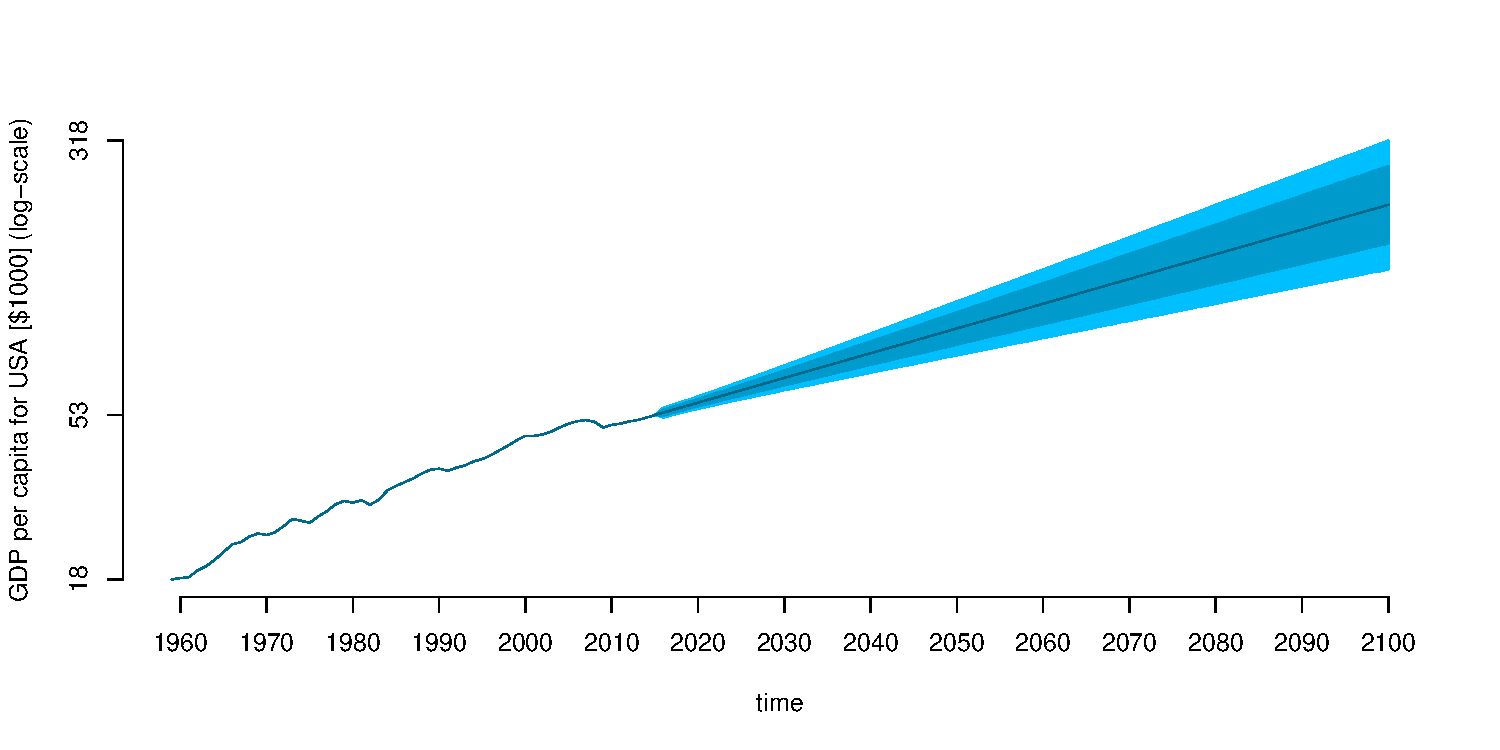
\includegraphics[trim=1cm 0cm 2cm 2cm, scale=0.4]{./01empirical/gdp-1-USA.pdf}

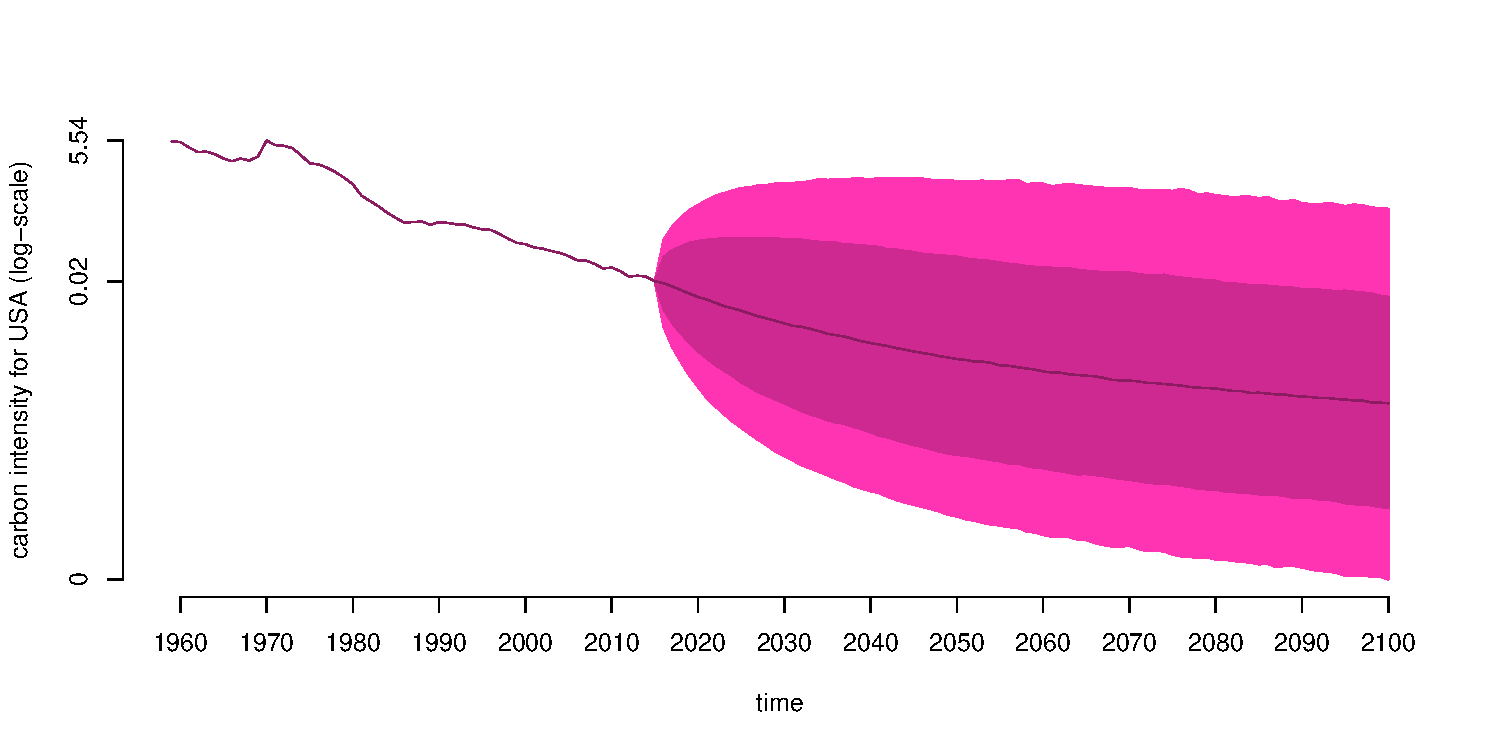
\includegraphics[trim=1cm 0cm 2cm 2cm, scale=0.4]{./01empirical/cie-1-USA.pdf}
\end{center}
\end{frame}



\begin{frame}{Predictions: Australia}

\begin{center}
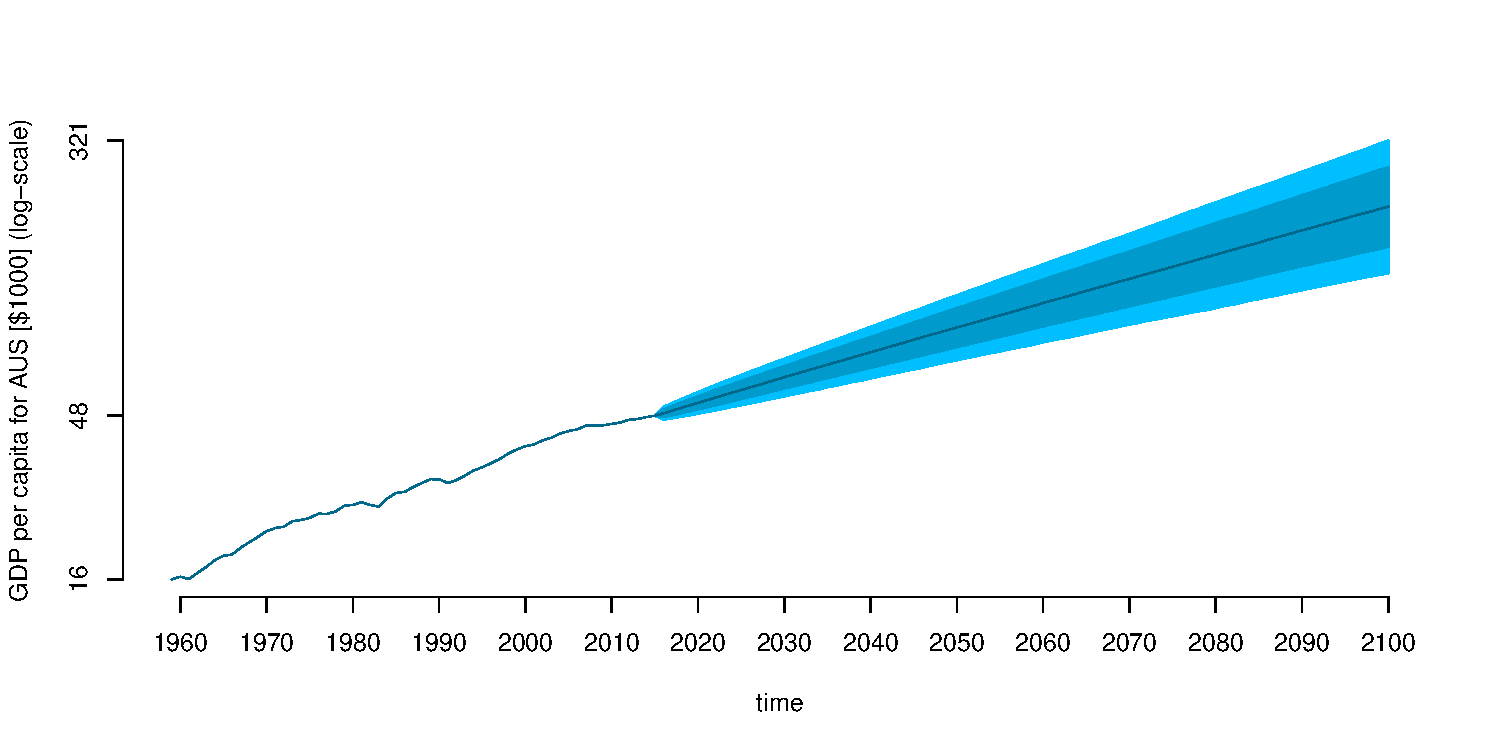
\includegraphics[trim=1cm 0cm 2cm 2cm, scale=0.4]{./01empirical/gdp-2-AUS.pdf}

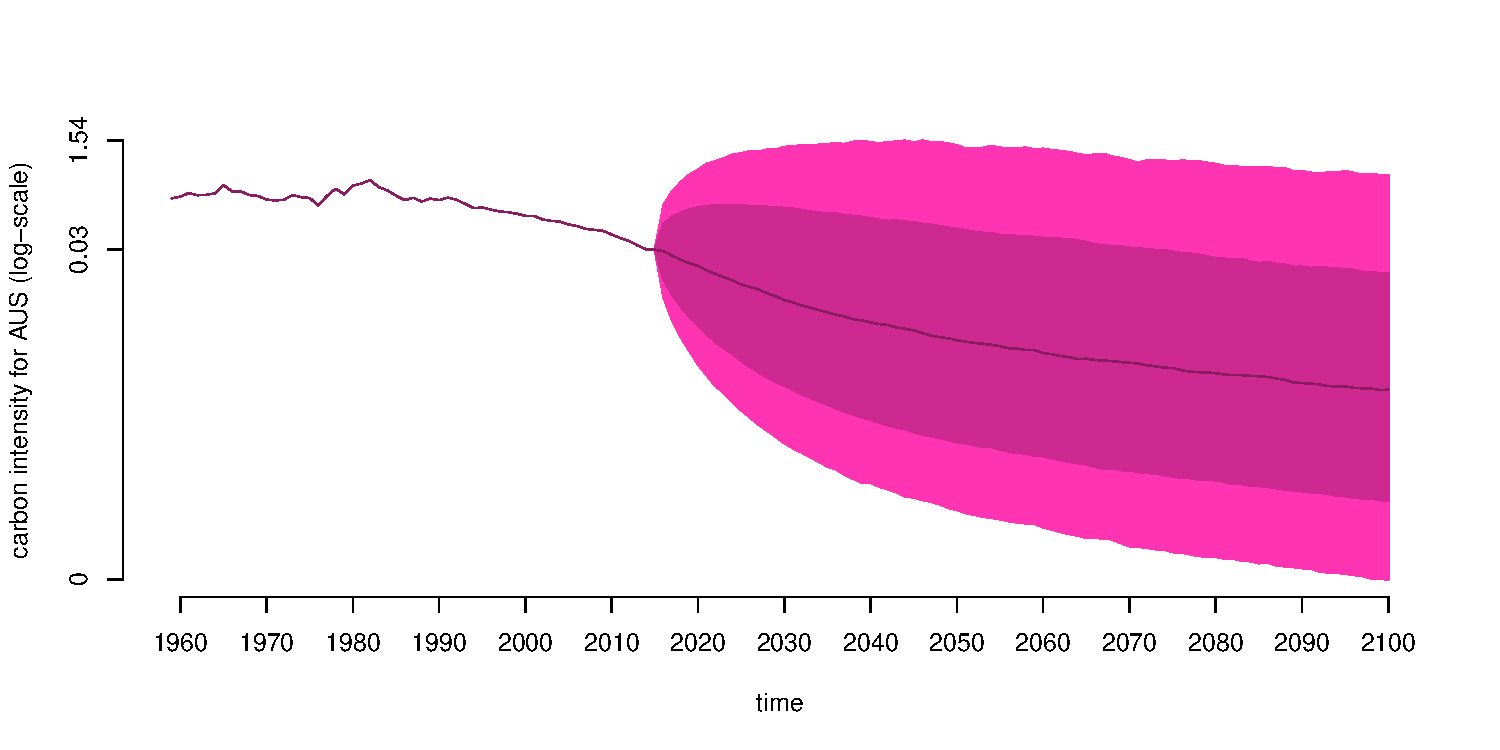
\includegraphics[trim=1cm 0cm 2cm 2cm, scale=0.4]{./01empirical/cie-2-AUS.pdf}

\end{center}
\end{frame}




\begin{frame}{Predictions: Canada}

\begin{center}
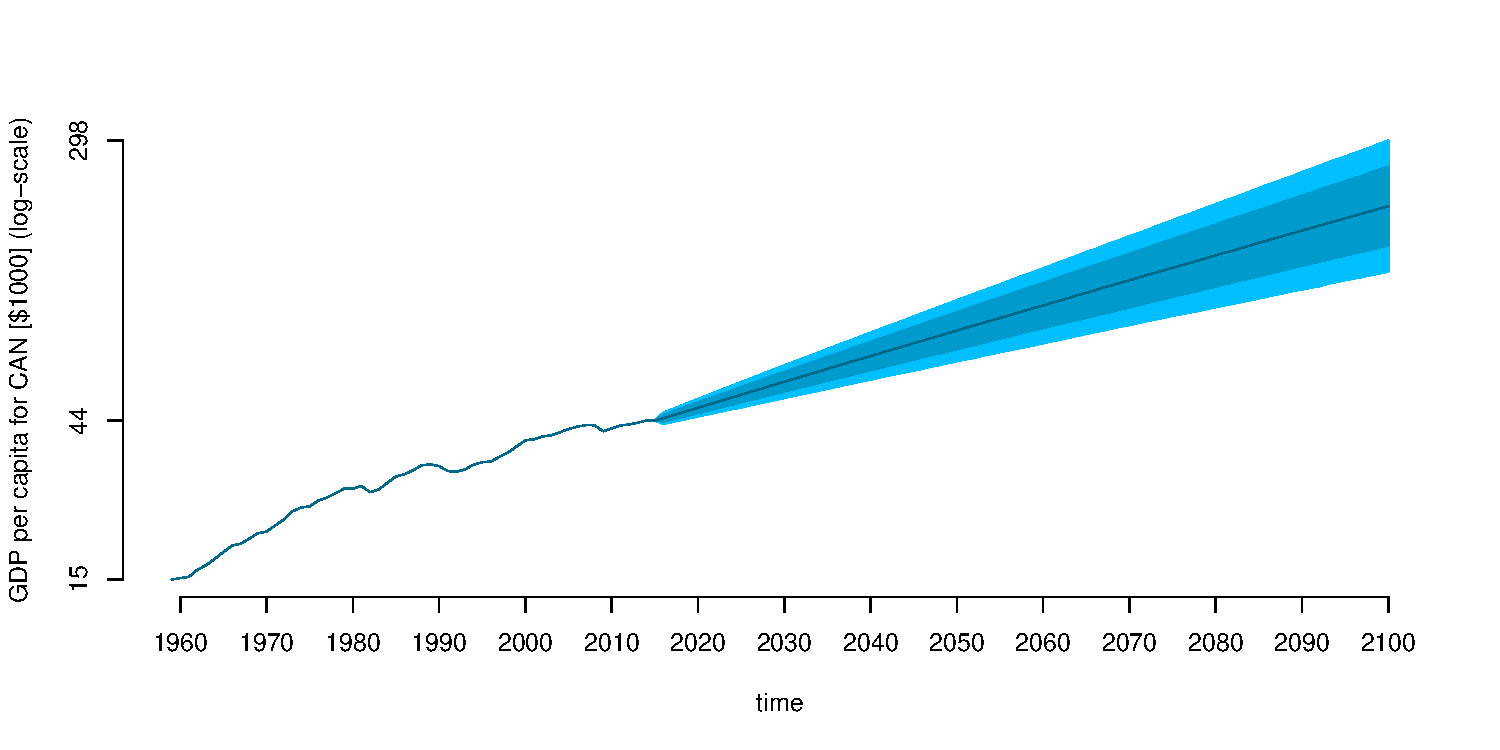
\includegraphics[trim=1cm 0cm 2cm 2cm, scale=0.4]{./01empirical/gdp-3-CAN.pdf}

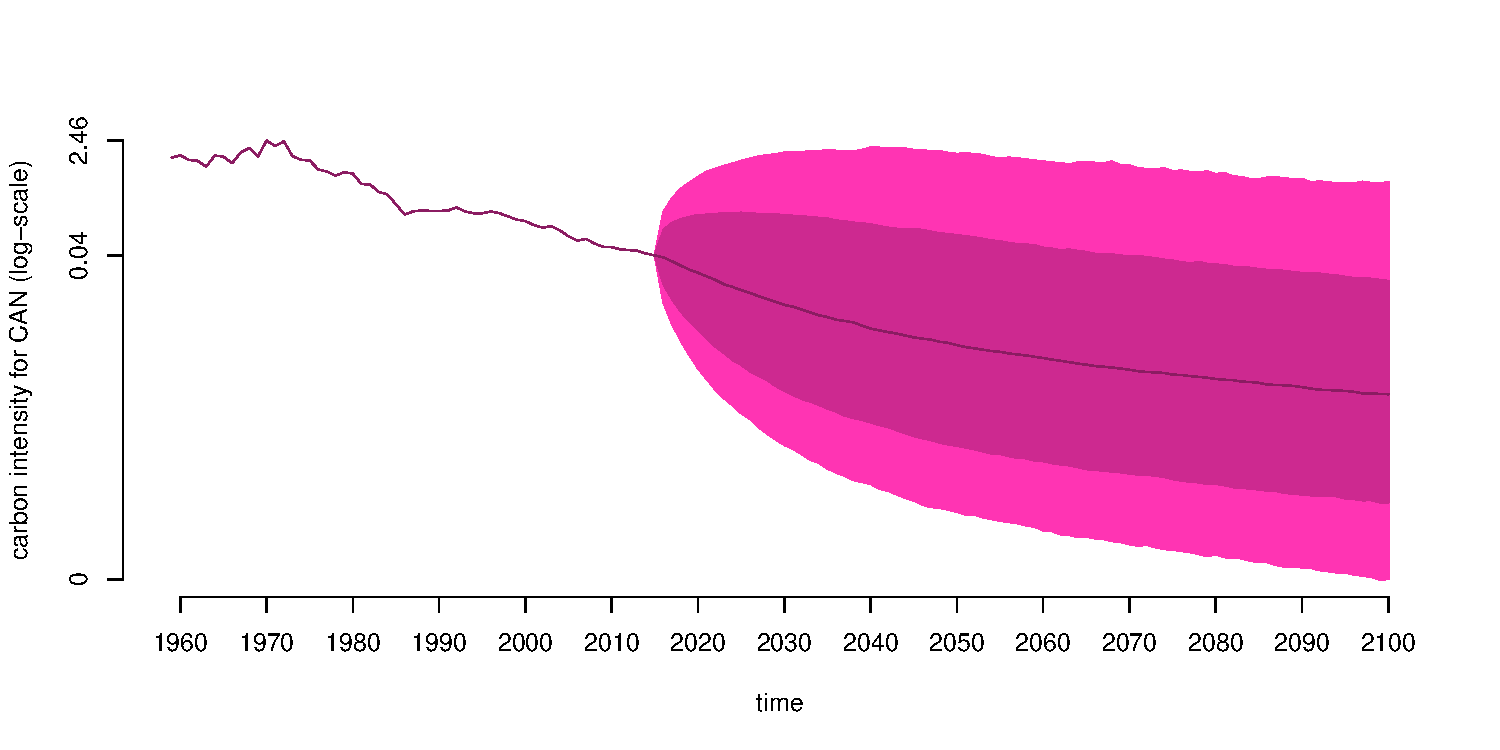
\includegraphics[trim=1cm 0cm 2cm 2cm, scale=0.4]{./01empirical/cie-3-CAN.pdf}
\end{center}
\end{frame}

\begin{frame}{Predictions: China}

\begin{center}
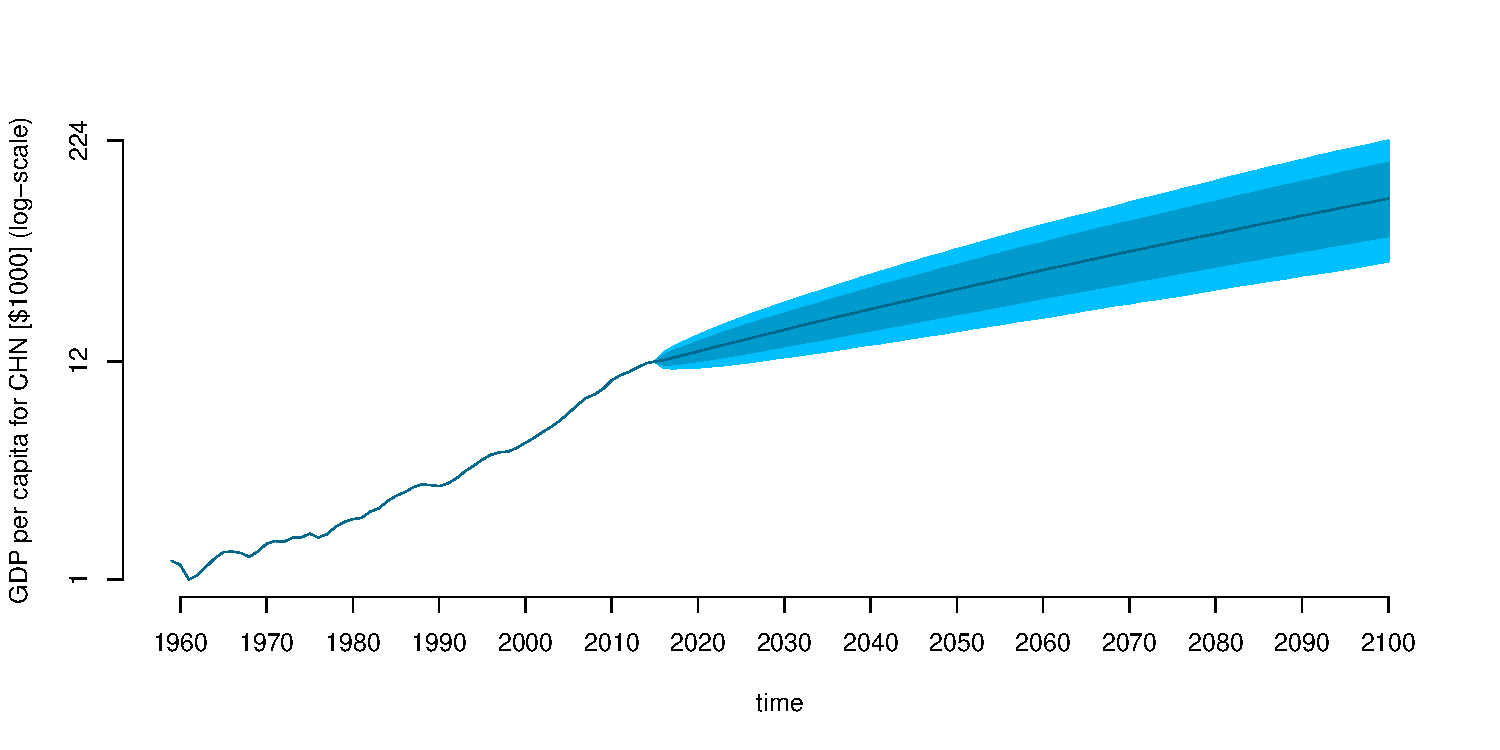
\includegraphics[trim=1cm 0cm 2cm 2cm, scale=0.4]{./01empirical/gdp-4-CHN.pdf}

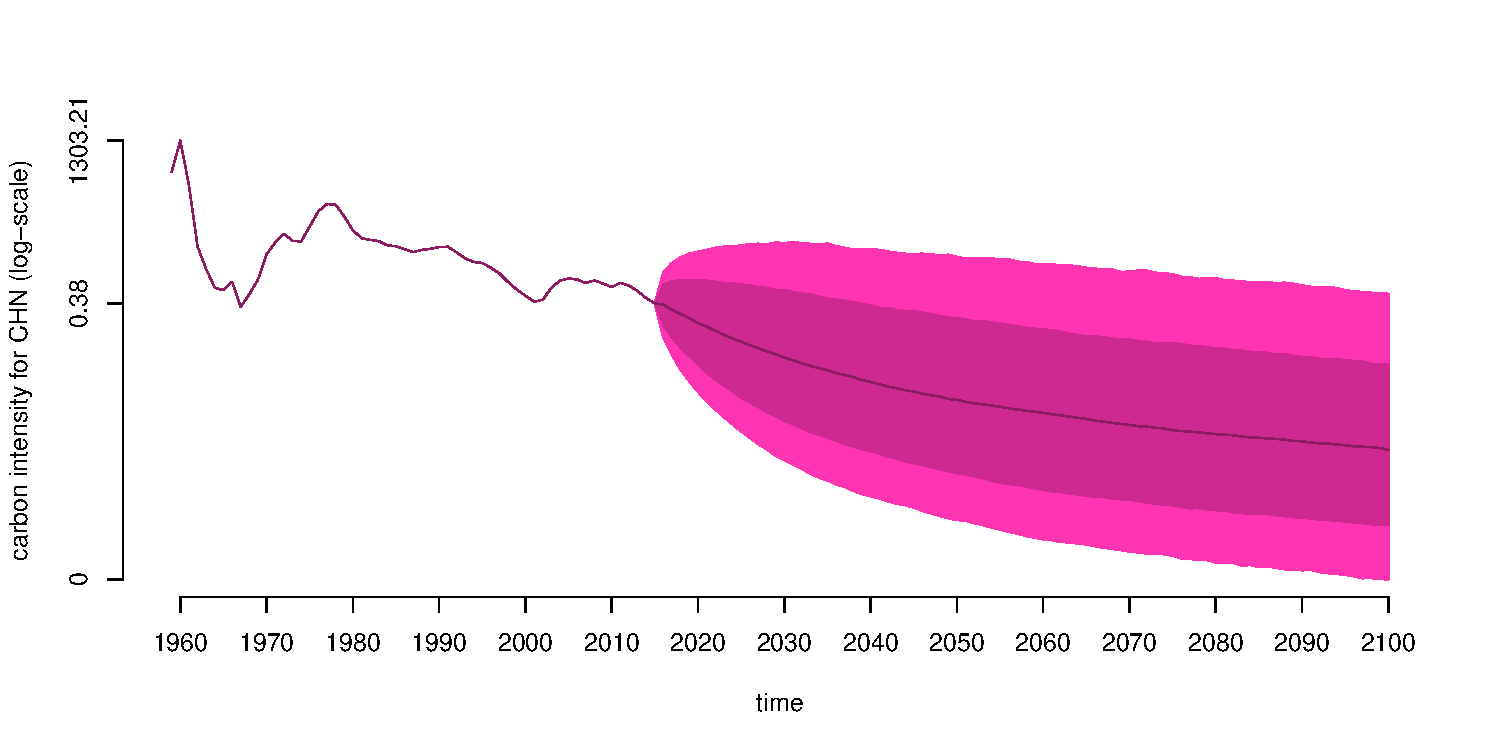
\includegraphics[trim=1cm 0cm 2cm 2cm, scale=0.4]{./01empirical/cie-4-CHN.pdf}
\end{center}
\end{frame}




\begin{frame}{Predictions: Indonesia}

\begin{center}
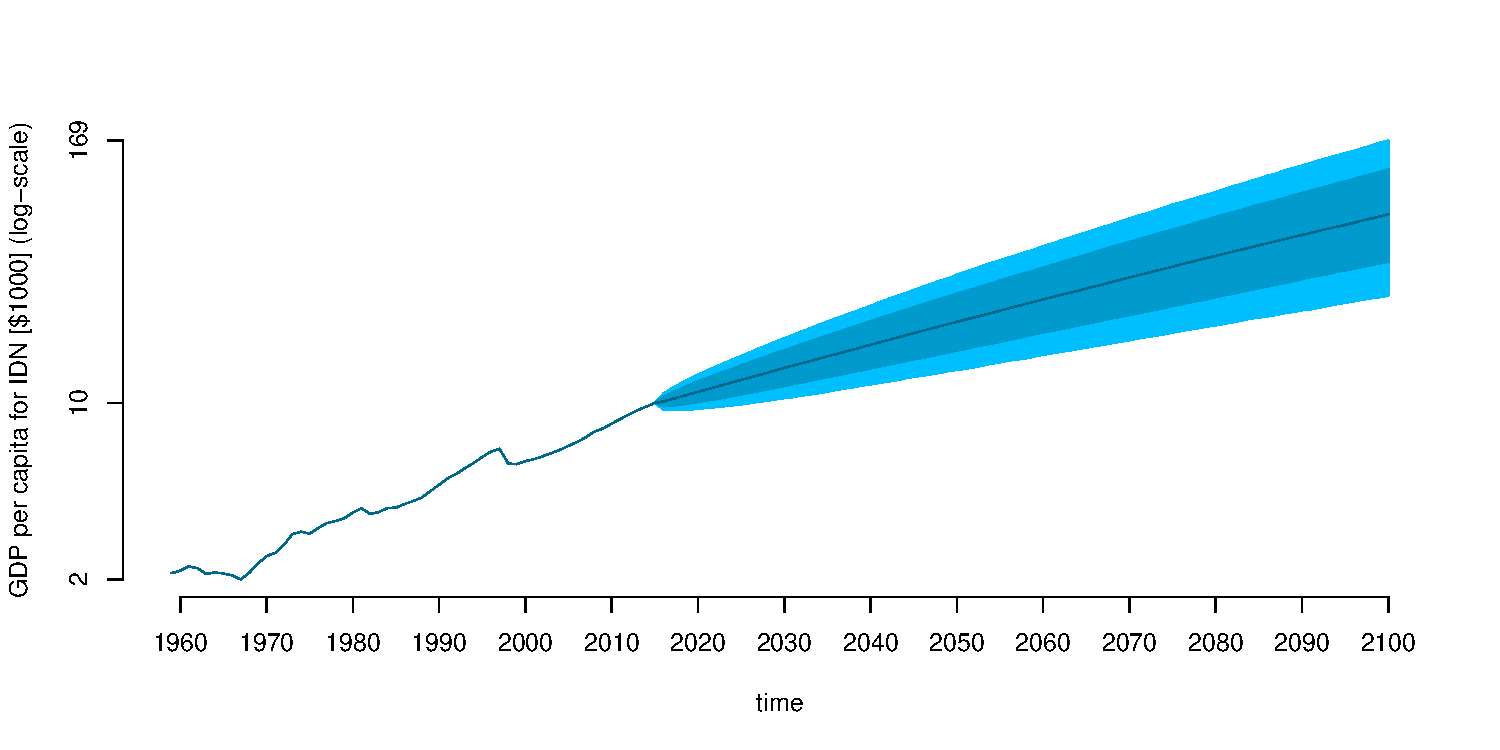
\includegraphics[trim=1cm 0cm 2cm 2cm, scale=0.4]{./01empirical/gdp-5-IDN.pdf}

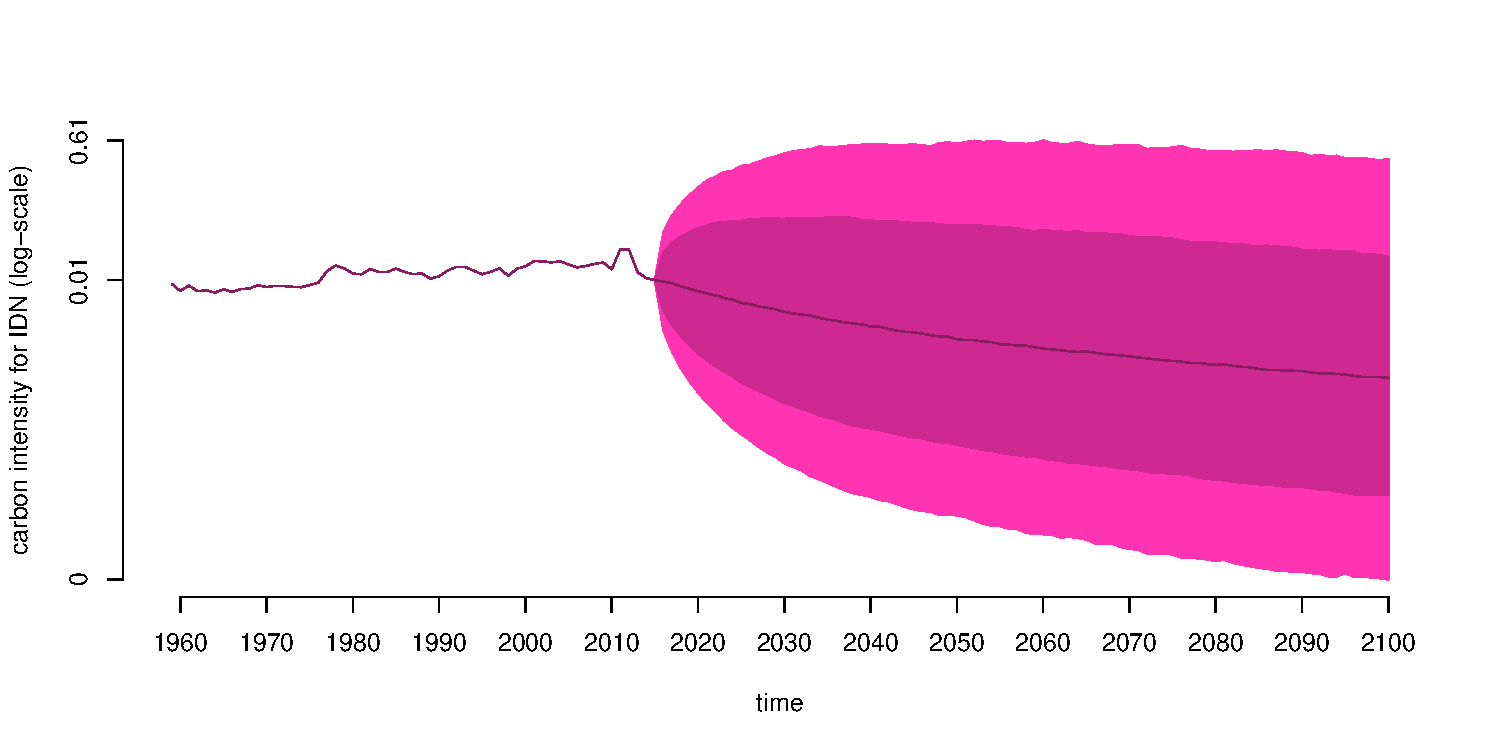
\includegraphics[trim=1cm 0cm 2cm 2cm, scale=0.4]{./01empirical/cie-5-IDN.pdf}
\end{center}
\end{frame}




\begin{frame}{Predictions: India}

\begin{center}
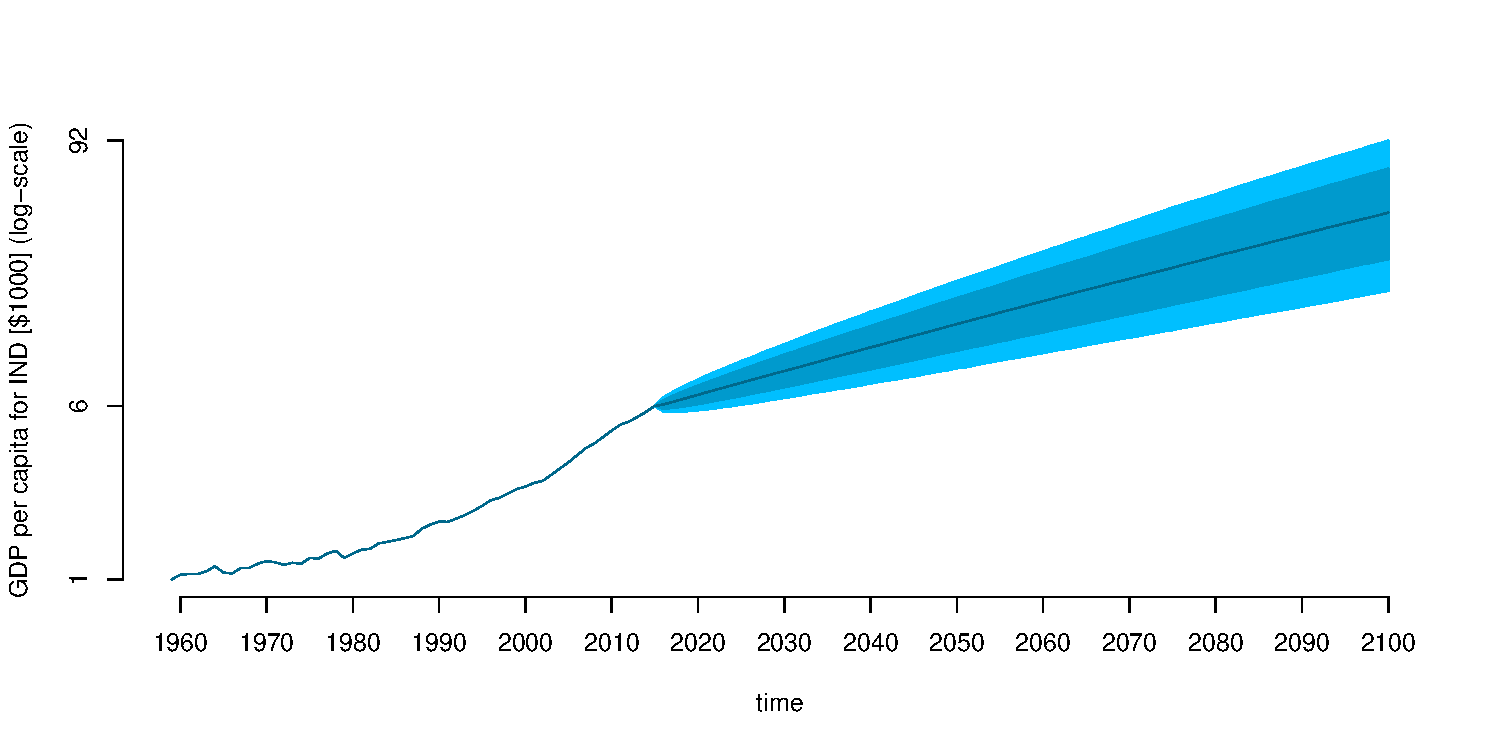
\includegraphics[trim=1cm 0cm 2cm 2cm, scale=0.4]{./01empirical/gdp-6-IND.pdf}

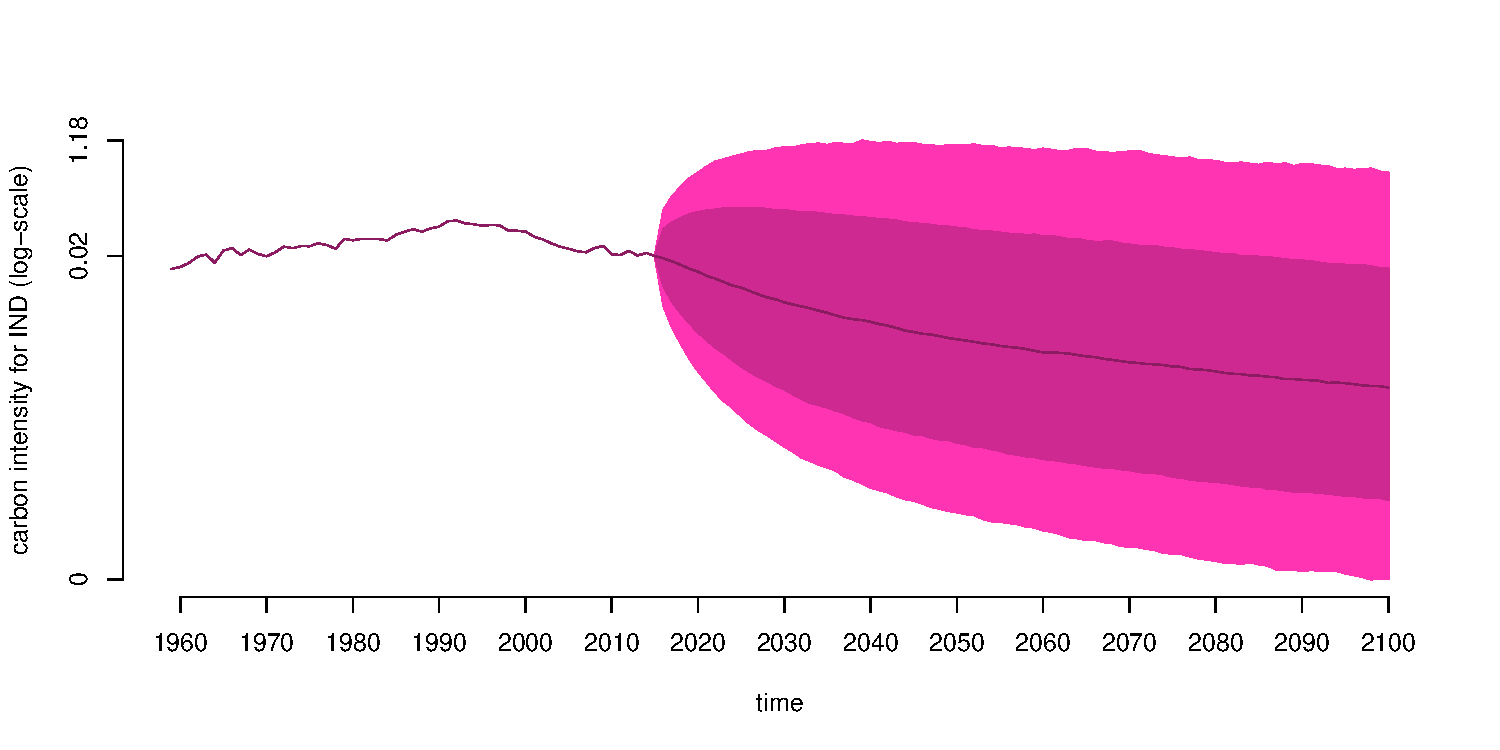
\includegraphics[trim=1cm 0cm 2cm 2cm, scale=0.4]{./01empirical/cie-6-IND.pdf}
\end{center}
\end{frame}



\begin{frame}{Predictions: Japan}

\begin{center}
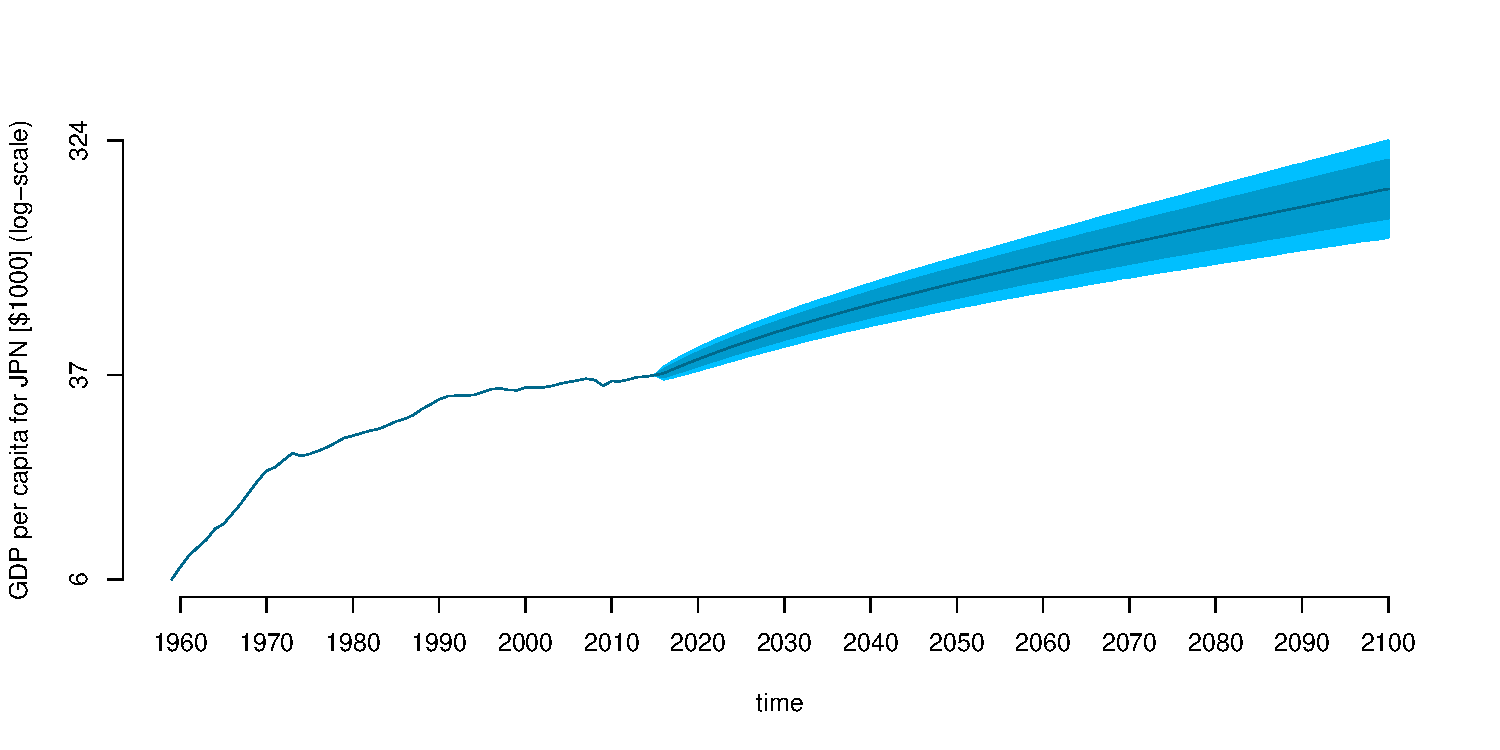
\includegraphics[trim=1cm 0cm 2cm 2cm, scale=0.4]{./01empirical/gdp-7-JPN.pdf}

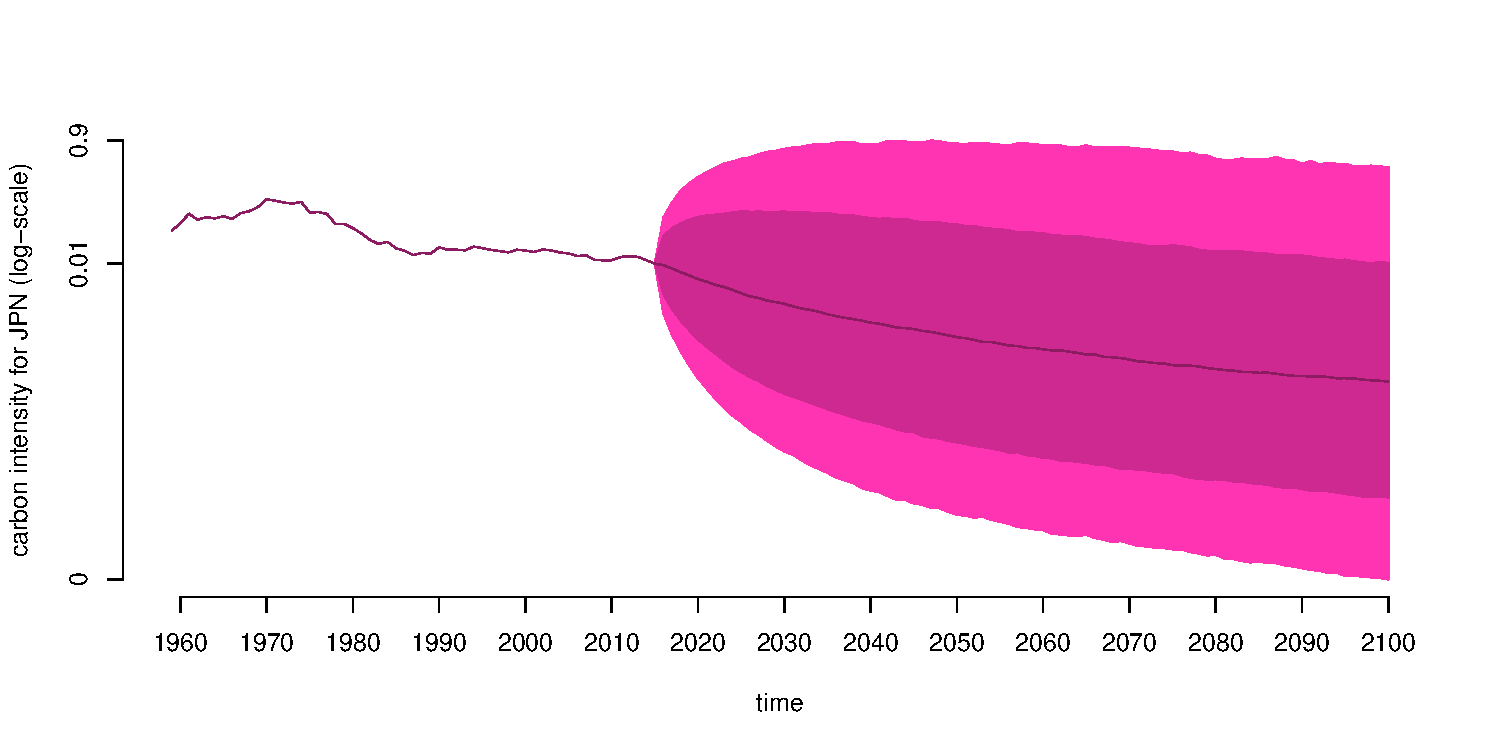
\includegraphics[trim=1cm 0cm 2cm 2cm, scale=0.4]{./01empirical/cie-7-JPN.pdf}
\end{center}
\end{frame}



\begin{frame}{Predictions: New Zealand}

\begin{center}
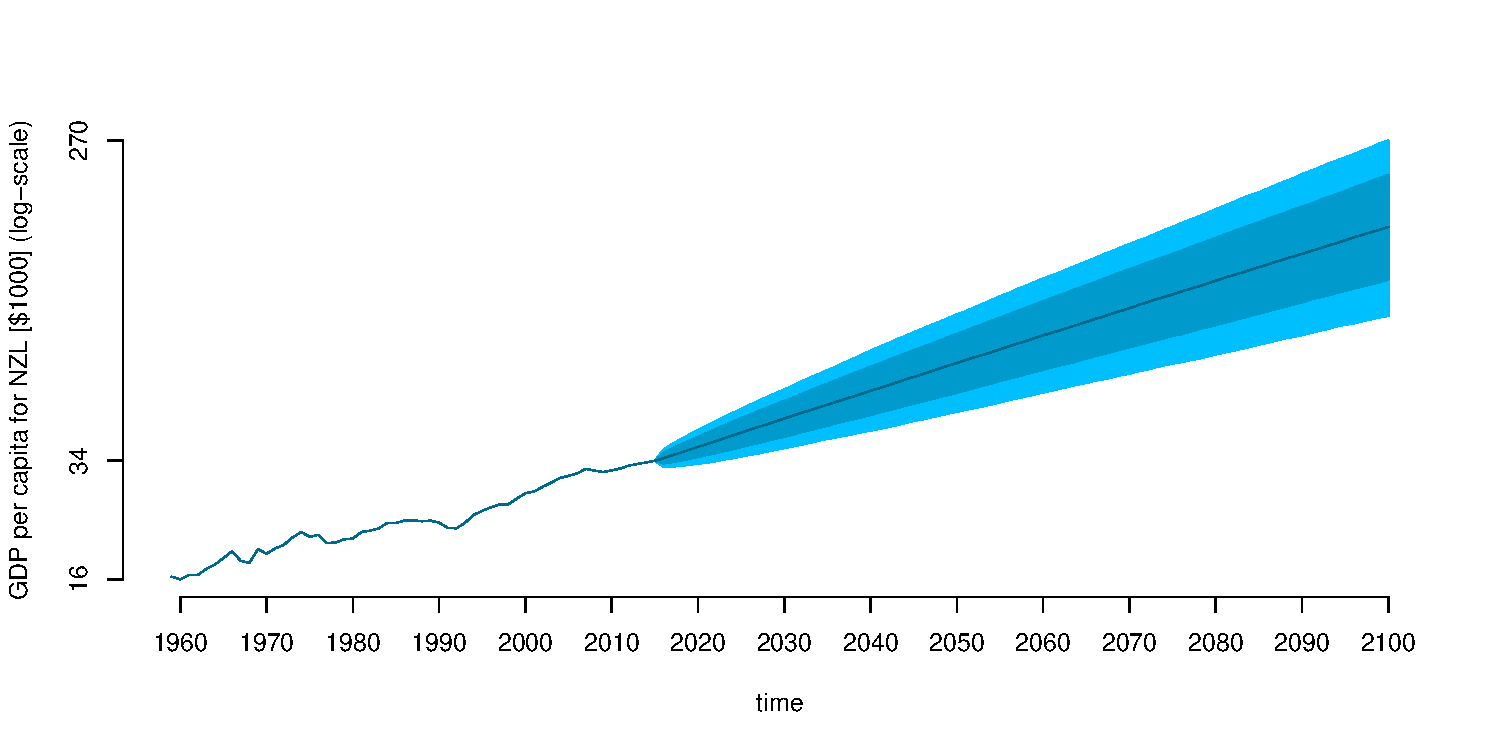
\includegraphics[trim=1cm 0cm 2cm 2cm, scale=0.4]{./01empirical/gdp-8-NZL.pdf}

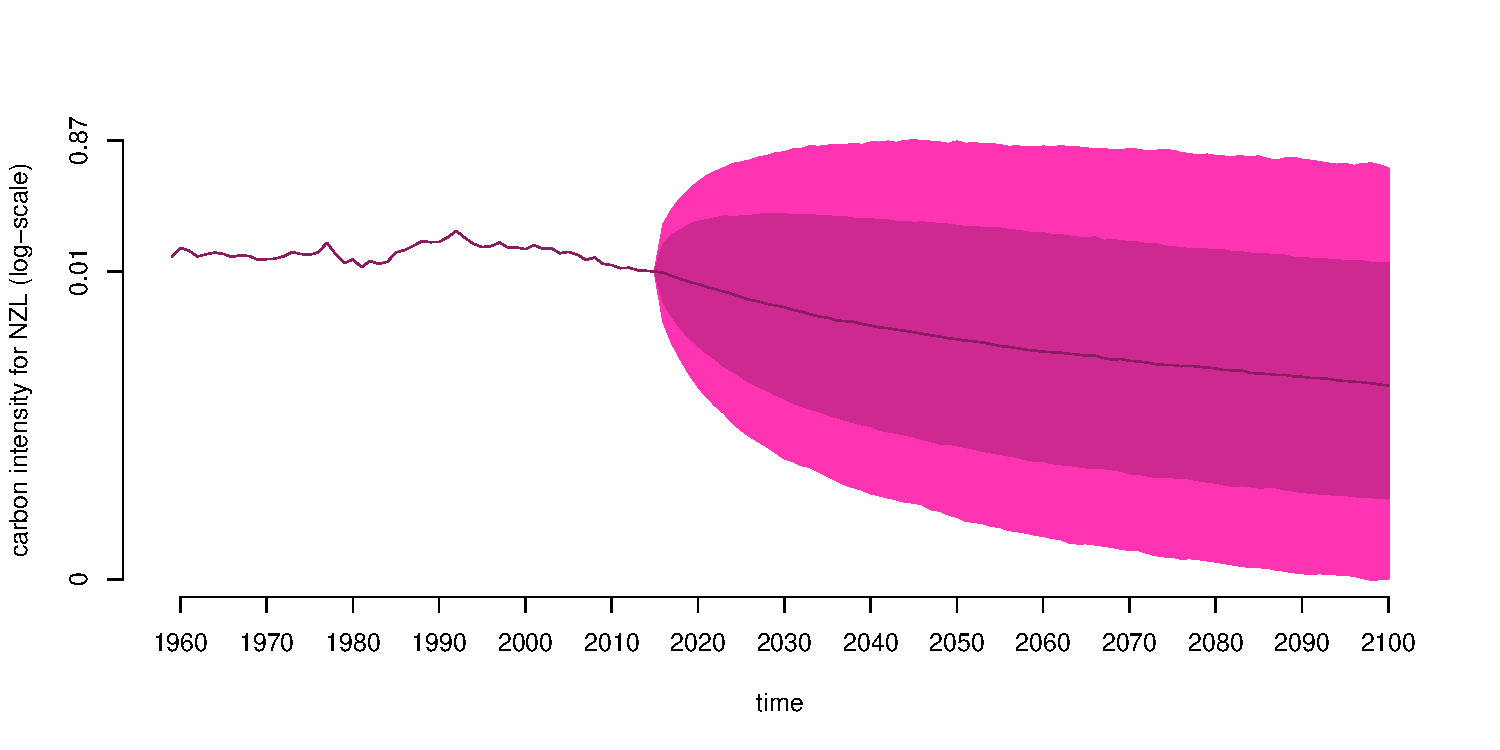
\includegraphics[trim=1cm 0cm 2cm 2cm, scale=0.4]{./01empirical/cie-8-NZL.pdf}
\end{center}
\end{frame}



\begin{frame}{Predictions: Philippines}

\begin{center}
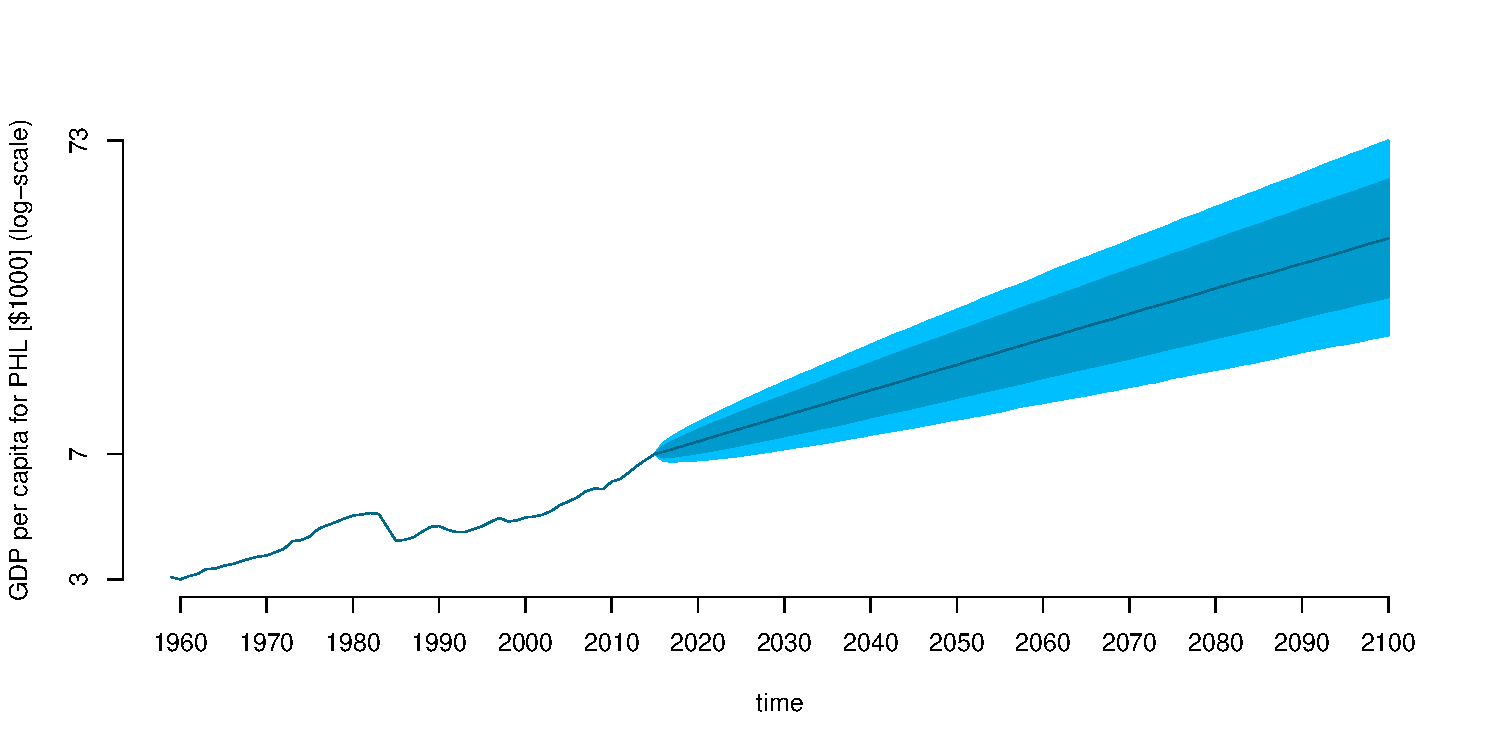
\includegraphics[trim=1cm 0cm 2cm 2cm, scale=0.4]{./01empirical/gdp-9-PHL.pdf}

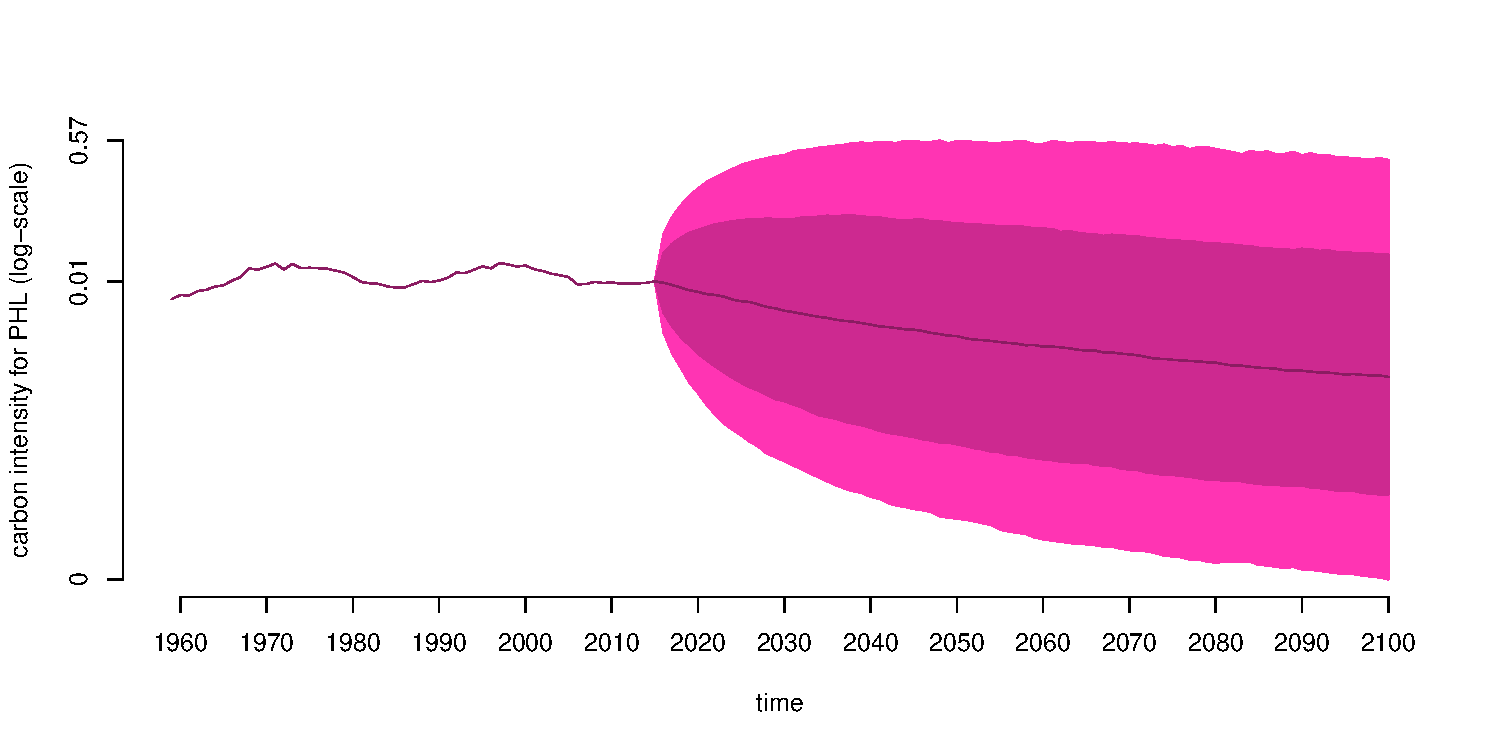
\includegraphics[trim=1cm 0cm 2cm 2cm, scale=0.4]{./01empirical/cie-9-PHL.pdf}
\end{center}
\end{frame}




\begin{frame}{Predictions: Poland}

\begin{center}
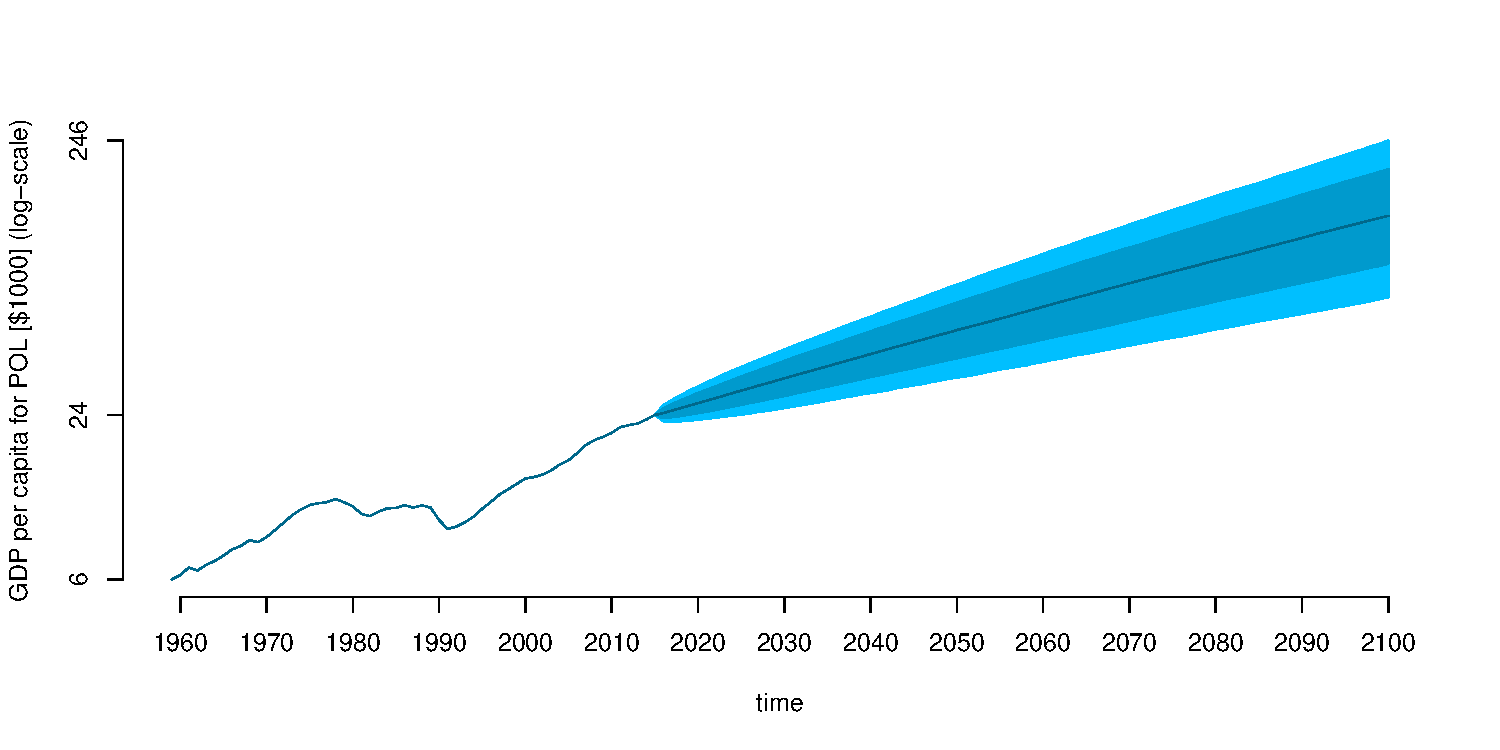
\includegraphics[trim=1cm 0cm 2cm 2cm, scale=0.4]{./01empirical/gdp-10-POL.pdf}

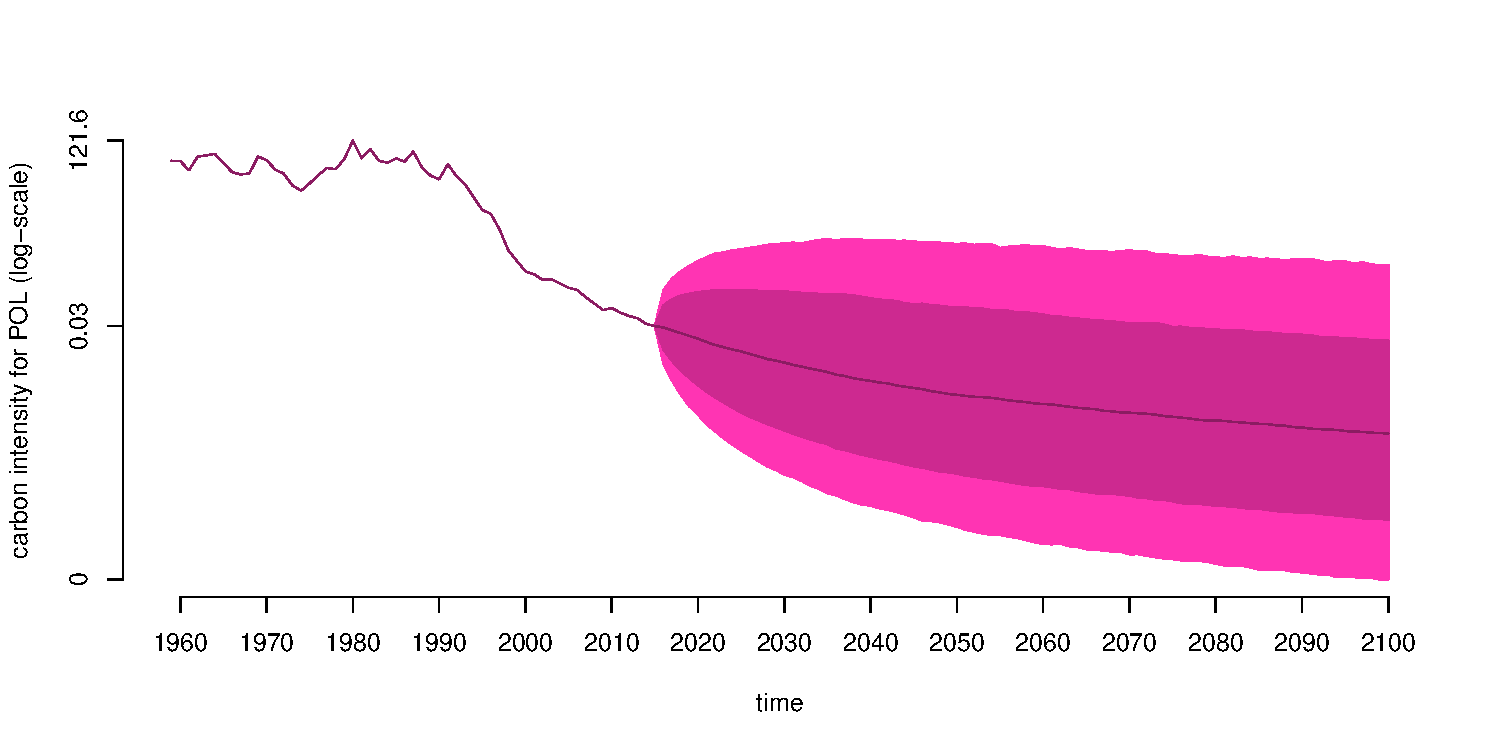
\includegraphics[trim=1cm 0cm 2cm 2cm, scale=0.4]{./01empirical/cie-10-POL.pdf}
\end{center}
\end{frame}


{\setbeamercolor{background canvas}{bg=gre}
\begin{frame}{\color{blu}Less than $2^{\circ}$C warming by 2100 unlikely}

\begin{description}
\item[\color{blu}Long-run forecasting] {\color{yel}of quantities that are essential for decision-makers faces multiple challenges} 

\bigskip\item[\color{blu}Probabilistic forecasting] {\color{yel}is crucial for realistic assessment of future tendencies } 

\bigskip\item[\color{blu}Hierarchical Bayesian] {\color{yel} modeling provides additional tools to calibrate the model to the objective of the research} 

\bigskip\item[\color{blu}Much stricter policies] {\color{yel}lowering the carbon intensity of economies are required to keep the increase in global temperatures below the level triggering multiple climate change tipping points}

\end{description}

\end{frame}}


\end{document} 